\documentclass[twoside]{book}

% Packages required by doxygen
\usepackage{calc}
\usepackage{doxygen}
\usepackage{graphicx}
\usepackage[utf8]{inputenc}
\usepackage{makeidx}
\usepackage{multicol}
\usepackage{multirow}
\usepackage{textcomp}
\usepackage[table]{xcolor}

% Font selection
\usepackage[T1]{fontenc}
\usepackage{mathptmx}
\usepackage[scaled=.90]{helvet}
\usepackage{courier}
\usepackage{amssymb}
\usepackage{sectsty}
\renewcommand{\familydefault}{\sfdefault}
\allsectionsfont{%
  \fontseries{bc}\selectfont%
  \color{darkgray}%
}
\renewcommand{\DoxyLabelFont}{%
  \fontseries{bc}\selectfont%
  \color{darkgray}%
}

% Page & text layout
\usepackage{geometry}
\geometry{%
  a4paper,%
  top=2.5cm,%
  bottom=2.5cm,%
  left=2.5cm,%
  right=2.5cm%
}
\tolerance=750
\hfuzz=15pt
\hbadness=750
\setlength{\emergencystretch}{15pt}
\setlength{\parindent}{0cm}
\setlength{\parskip}{0.2cm}
\makeatletter
\renewcommand{\paragraph}{%
  \@startsection{paragraph}{4}{0ex}{-1.0ex}{1.0ex}{%
    \normalfont\normalsize\bfseries\SS@parafont%
  }%
}
\renewcommand{\subparagraph}{%
  \@startsection{subparagraph}{5}{0ex}{-1.0ex}{1.0ex}{%
    \normalfont\normalsize\bfseries\SS@subparafont%
  }%
}
\makeatother

% Headers & footers
\usepackage{fancyhdr}
\pagestyle{fancyplain}
\fancyhead[LE]{\fancyplain{}{\bfseries\thepage}}
\fancyhead[CE]{\fancyplain{}{}}
\fancyhead[RE]{\fancyplain{}{\bfseries\leftmark}}
\fancyhead[LO]{\fancyplain{}{\bfseries\rightmark}}
\fancyhead[CO]{\fancyplain{}{}}
\fancyhead[RO]{\fancyplain{}{\bfseries\thepage}}
\fancyfoot[LE]{\fancyplain{}{}}
\fancyfoot[CE]{\fancyplain{}{}}
\fancyfoot[RE]{\fancyplain{}{\bfseries\scriptsize Generated on Thu Mar 5 2015 09\-:49\-:34 by Doxygen }}
\fancyfoot[LO]{\fancyplain{}{\bfseries\scriptsize Generated on Thu Mar 5 2015 09\-:49\-:34 by Doxygen }}
\fancyfoot[CO]{\fancyplain{}{}}
\fancyfoot[RO]{\fancyplain{}{}}
\renewcommand{\footrulewidth}{0.4pt}
\renewcommand{\chaptermark}[1]{%
  \markboth{#1}{}%
}
\renewcommand{\sectionmark}[1]{%
  \markright{\thesection\ #1}%
}

% Indices & bibliography
\usepackage{natbib}
\usepackage[titles]{tocloft}
\setcounter{tocdepth}{3}
\setcounter{secnumdepth}{5}
\makeindex

% Hyperlinks (required, but should be loaded last)
\usepackage{ifpdf}
\ifpdf
  \usepackage[pdftex,pagebackref=true]{hyperref}
\else
  \usepackage[ps2pdf,pagebackref=true]{hyperref}
\fi
\hypersetup{%
  colorlinks=true,%
  linkcolor=blue,%
  citecolor=blue,%
  unicode%
}

% Custom commands
\newcommand{\clearemptydoublepage}{%
  \newpage{\pagestyle{empty}\cleardoublepage}%
}


%===== C O N T E N T S =====

\begin{document}

% Titlepage & ToC
\hypersetup{pageanchor=false}
\pagenumbering{roman}
\begin{titlepage}
\vspace*{7cm}
\begin{center}%
{\Large Reference Manual}\\
\vspace*{1cm}
{\large Generated by Doxygen 1.8.6}\\
\vspace*{0.5cm}
{\small Thu Mar 5 2015 09:49:34}\\
\end{center}
\end{titlepage}
\clearemptydoublepage
\tableofcontents
\clearemptydoublepage
\pagenumbering{arabic}
\hypersetup{pageanchor=true}

%--- Begin generated contents ---
\chapter{Hierarchical Index}
\section{Class Hierarchy}
This inheritance list is sorted roughly, but not completely, alphabetically\-:\begin{DoxyCompactList}
\item F\-S\-M\-Context\begin{DoxyCompactList}
\item \contentsline{section}{cpp\-Context}{\pageref{classcpp_context}}{}
\item \contentsline{section}{sal\-Lifecycle\-\_\-sm.\-sal\-Lifecycle\-\_\-sm}{\pageref{classsal_lifecycle__sm_1_1sal_lifecycle__sm}}{}
\item \contentsline{section}{sal\-Lifecycle\-Context}{\pageref{classsal_lifecycle_context}}{}
\end{DoxyCompactList}
\item \contentsline{section}{Main\-Map}{\pageref{class_main_map}}{}
\item object\begin{DoxyCompactList}
\item \contentsline{section}{sal\-Lifecycle\-\_\-sm.\-Main\-Map}{\pageref{classsal_lifecycle__sm_1_1_main_map}}{}
\end{DoxyCompactList}
\item State\begin{DoxyCompactList}
\item \contentsline{section}{sal\-Lifecycle\-\_\-sm.\-sal\-Lifecycle\-State}{\pageref{classsal_lifecycle__sm_1_1sal_lifecycle_state}}{}
\begin{DoxyCompactList}
\item \contentsline{section}{sal\-Lifecycle\-\_\-sm.\-Main\-Map\-\_\-\-Default}{\pageref{classsal_lifecycle__sm_1_1_main_map___default}}{}
\begin{DoxyCompactList}
\item \contentsline{section}{sal\-Lifecycle\-\_\-sm.\-Main\-Map\-\_\-\-C\-O\-N\-F\-I\-G\-U\-R\-I\-N\-G}{\pageref{classsal_lifecycle__sm_1_1_main_map___c_o_n_f_i_g_u_r_i_n_g}}{}
\item \contentsline{section}{sal\-Lifecycle\-\_\-sm.\-Main\-Map\-\_\-\-D\-I\-S\-A\-B\-L\-E\-D}{\pageref{classsal_lifecycle__sm_1_1_main_map___d_i_s_a_b_l_e_d}}{}
\item \contentsline{section}{sal\-Lifecycle\-\_\-sm.\-Main\-Map\-\_\-\-E\-N\-A\-B\-L\-E\-D}{\pageref{classsal_lifecycle__sm_1_1_main_map___e_n_a_b_l_e_d}}{}
\item \contentsline{section}{sal\-Lifecycle\-\_\-sm.\-Main\-Map\-\_\-\-E\-R\-R\-O\-R}{\pageref{classsal_lifecycle__sm_1_1_main_map___e_r_r_o_r}}{}
\item \contentsline{section}{sal\-Lifecycle\-\_\-sm.\-Main\-Map\-\_\-\-Off}{\pageref{classsal_lifecycle__sm_1_1_main_map___off}}{}
\item \contentsline{section}{sal\-Lifecycle\-\_\-sm.\-Main\-Map\-\_\-\-S\-T\-A\-N\-D\-B\-Y}{\pageref{classsal_lifecycle__sm_1_1_main_map___s_t_a_n_d_b_y}}{}
\end{DoxyCompactList}
\end{DoxyCompactList}
\item \contentsline{section}{sal\-Lifecycle\-State}{\pageref{classsal_lifecycle_state}}{}
\begin{DoxyCompactList}
\item \contentsline{section}{Main\-Map\-\_\-\-Default}{\pageref{class_main_map___default}}{}
\begin{DoxyCompactList}
\item \contentsline{section}{Main\-Map\-\_\-\-C\-O\-N\-F\-I\-G\-U\-R\-I\-N\-G}{\pageref{class_main_map___c_o_n_f_i_g_u_r_i_n_g}}{}
\item \contentsline{section}{Main\-Map\-\_\-\-D\-I\-S\-A\-B\-L\-E\-D}{\pageref{class_main_map___d_i_s_a_b_l_e_d}}{}
\item \contentsline{section}{Main\-Map\-\_\-\-E\-N\-A\-B\-L\-E\-D}{\pageref{class_main_map___e_n_a_b_l_e_d}}{}
\item \contentsline{section}{Main\-Map\-\_\-\-E\-R\-R\-O\-R}{\pageref{class_main_map___e_r_r_o_r}}{}
\item \contentsline{section}{Main\-Map\-\_\-\-Off}{\pageref{class_main_map___off}}{}
\item \contentsline{section}{Main\-Map\-\_\-\-S\-T\-A\-N\-D\-B\-Y}{\pageref{class_main_map___s_t_a_n_d_b_y}}{}
\end{DoxyCompactList}
\end{DoxyCompactList}
\end{DoxyCompactList}
\end{DoxyCompactList}

\chapter{Class Index}
\section{Class List}
Here are the classes, structs, unions and interfaces with brief descriptions\-:\begin{DoxyCompactList}
\item\contentsline{section}{\hyperlink{classcpp_context}{cpp\-Context} }{\pageref{classcpp_context}}{}
\item\contentsline{section}{\hyperlink{class_main_map}{Main\-Map} }{\pageref{class_main_map}}{}
\item\contentsline{section}{\hyperlink{classsal_lifecycle__sm_1_1_main_map}{sal\-Lifecycle\-\_\-sm.\-Main\-Map} }{\pageref{classsal_lifecycle__sm_1_1_main_map}}{}
\item\contentsline{section}{\hyperlink{class_main_map___c_o_n_f_i_g_u_r_i_n_g}{Main\-Map\-\_\-\-C\-O\-N\-F\-I\-G\-U\-R\-I\-N\-G} }{\pageref{class_main_map___c_o_n_f_i_g_u_r_i_n_g}}{}
\item\contentsline{section}{\hyperlink{classsal_lifecycle__sm_1_1_main_map___c_o_n_f_i_g_u_r_i_n_g}{sal\-Lifecycle\-\_\-sm.\-Main\-Map\-\_\-\-C\-O\-N\-F\-I\-G\-U\-R\-I\-N\-G} }{\pageref{classsal_lifecycle__sm_1_1_main_map___c_o_n_f_i_g_u_r_i_n_g}}{}
\item\contentsline{section}{\hyperlink{classsal_lifecycle__sm_1_1_main_map___default}{sal\-Lifecycle\-\_\-sm.\-Main\-Map\-\_\-\-Default} }{\pageref{classsal_lifecycle__sm_1_1_main_map___default}}{}
\item\contentsline{section}{\hyperlink{class_main_map___default}{Main\-Map\-\_\-\-Default} }{\pageref{class_main_map___default}}{}
\item\contentsline{section}{\hyperlink{classsal_lifecycle__sm_1_1_main_map___d_i_s_a_b_l_e_d}{sal\-Lifecycle\-\_\-sm.\-Main\-Map\-\_\-\-D\-I\-S\-A\-B\-L\-E\-D} }{\pageref{classsal_lifecycle__sm_1_1_main_map___d_i_s_a_b_l_e_d}}{}
\item\contentsline{section}{\hyperlink{class_main_map___d_i_s_a_b_l_e_d}{Main\-Map\-\_\-\-D\-I\-S\-A\-B\-L\-E\-D} }{\pageref{class_main_map___d_i_s_a_b_l_e_d}}{}
\item\contentsline{section}{\hyperlink{class_main_map___e_n_a_b_l_e_d}{Main\-Map\-\_\-\-E\-N\-A\-B\-L\-E\-D} }{\pageref{class_main_map___e_n_a_b_l_e_d}}{}
\item\contentsline{section}{\hyperlink{classsal_lifecycle__sm_1_1_main_map___e_n_a_b_l_e_d}{sal\-Lifecycle\-\_\-sm.\-Main\-Map\-\_\-\-E\-N\-A\-B\-L\-E\-D} }{\pageref{classsal_lifecycle__sm_1_1_main_map___e_n_a_b_l_e_d}}{}
\item\contentsline{section}{\hyperlink{class_main_map___e_r_r_o_r}{Main\-Map\-\_\-\-E\-R\-R\-O\-R} }{\pageref{class_main_map___e_r_r_o_r}}{}
\item\contentsline{section}{\hyperlink{classsal_lifecycle__sm_1_1_main_map___e_r_r_o_r}{sal\-Lifecycle\-\_\-sm.\-Main\-Map\-\_\-\-E\-R\-R\-O\-R} }{\pageref{classsal_lifecycle__sm_1_1_main_map___e_r_r_o_r}}{}
\item\contentsline{section}{\hyperlink{class_main_map___off}{Main\-Map\-\_\-\-Off} }{\pageref{class_main_map___off}}{}
\item\contentsline{section}{\hyperlink{classsal_lifecycle__sm_1_1_main_map___off}{sal\-Lifecycle\-\_\-sm.\-Main\-Map\-\_\-\-Off} }{\pageref{classsal_lifecycle__sm_1_1_main_map___off}}{}
\item\contentsline{section}{\hyperlink{class_main_map___s_t_a_n_d_b_y}{Main\-Map\-\_\-\-S\-T\-A\-N\-D\-B\-Y} }{\pageref{class_main_map___s_t_a_n_d_b_y}}{}
\item\contentsline{section}{\hyperlink{classsal_lifecycle__sm_1_1_main_map___s_t_a_n_d_b_y}{sal\-Lifecycle\-\_\-sm.\-Main\-Map\-\_\-\-S\-T\-A\-N\-D\-B\-Y} }{\pageref{classsal_lifecycle__sm_1_1_main_map___s_t_a_n_d_b_y}}{}
\item\contentsline{section}{\hyperlink{classsal_lifecycle__sm_1_1sal_lifecycle__sm}{sal\-Lifecycle\-\_\-sm.\-sal\-Lifecycle\-\_\-sm} }{\pageref{classsal_lifecycle__sm_1_1sal_lifecycle__sm}}{}
\item\contentsline{section}{\hyperlink{classsal_lifecycle_context}{sal\-Lifecycle\-Context} }{\pageref{classsal_lifecycle_context}}{}
\item\contentsline{section}{\hyperlink{classsal_lifecycle__sm_1_1sal_lifecycle_state}{sal\-Lifecycle\-\_\-sm.\-sal\-Lifecycle\-State} }{\pageref{classsal_lifecycle__sm_1_1sal_lifecycle_state}}{}
\item\contentsline{section}{\hyperlink{classsal_lifecycle_state}{sal\-Lifecycle\-State} }{\pageref{classsal_lifecycle_state}}{}
\end{DoxyCompactList}

\chapter{Class Documentation}
\hypertarget{classcpp_context}{\section{cpp\-Context Class Reference}
\label{classcpp_context}\index{cpp\-Context@{cpp\-Context}}
}
Inheritance diagram for cpp\-Context\-:\begin{figure}[H]
\begin{center}
\leavevmode
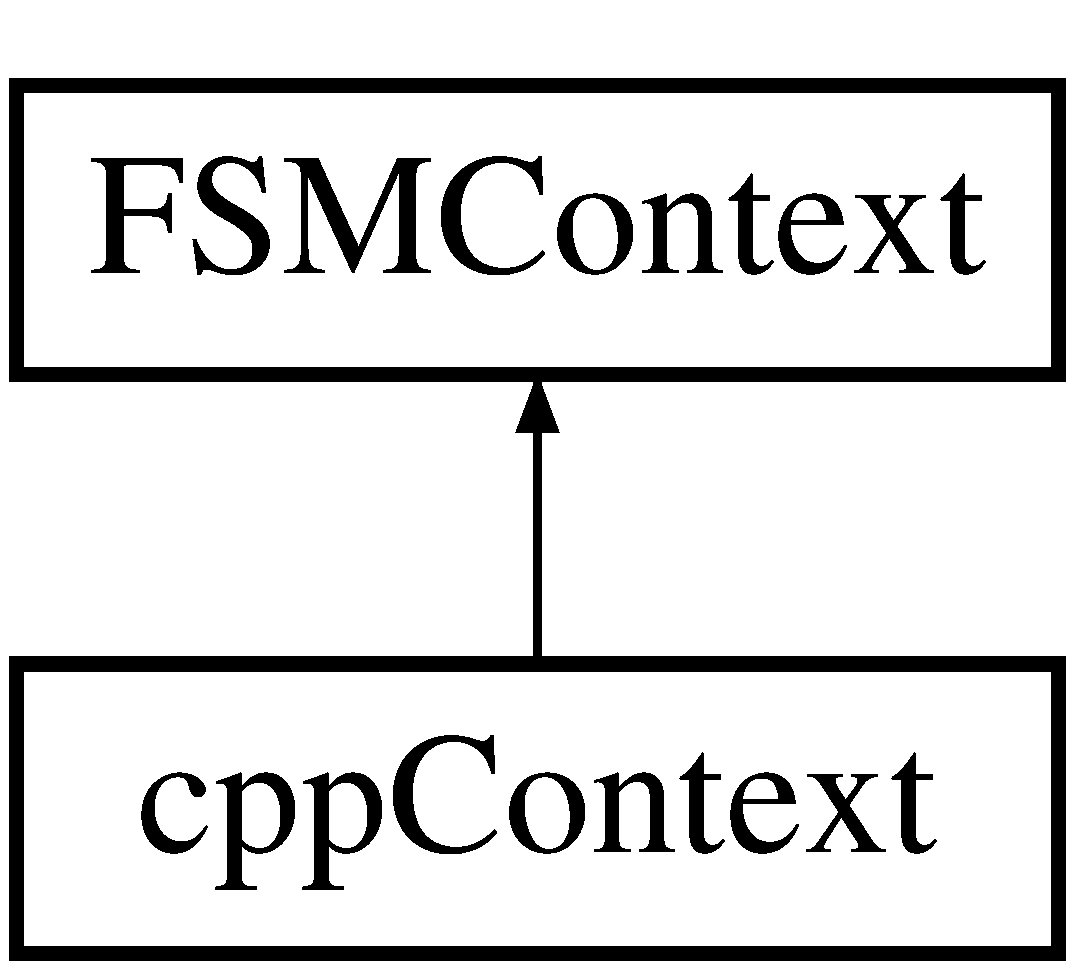
\includegraphics[height=2.000000cm]{classcpp_context}
\end{center}
\end{figure}
\subsection*{Public Member Functions}
\begin{DoxyCompactItemize}
\item 
\hypertarget{classcpp_context_adafe7a058dd5d2ae9aa4bb6fc0063a15}{sal\-Lifecycle {\bfseries cpp\-Context} (sal\-Lifecycle \&owner)}\label{classcpp_context_adafe7a058dd5d2ae9aa4bb6fc0063a15}

\item 
\hypertarget{classcpp_context_a75ccf2f8927f03c4bd6df6dda5d575b5}{sal\-Lifecycle {\bfseries cpp\-Context} (sal\-Lifecycle \&owner, const statemap\-::\-State \&state)}\label{classcpp_context_a75ccf2f8927f03c4bd6df6dda5d575b5}

\item 
\hypertarget{classcpp_context_a06ec75da099c8bedbd5f589af33c3c9b}{virtual void {\bfseries enter\-Start\-State} ()}\label{classcpp_context_a06ec75da099c8bedbd5f589af33c3c9b}

\item 
\hypertarget{classcpp_context_a7ede22c753aff55534ba826607c1798e}{sal\-Lifecycle \& {\bfseries get\-Owner} ()}\label{classcpp_context_a7ede22c753aff55534ba826607c1798e}

\item 
\hypertarget{classcpp_context_a0e71bb4ab685eb3c6dd458002868f597}{\hyperlink{classsal_lifecycle_state}{sal\-Lifecycle\-State} \& {\bfseries get\-State} ()}\label{classcpp_context_a0e71bb4ab685eb3c6dd458002868f597}

\item 
\hypertarget{classcpp_context_aeb607d9b38a25a3daa8eafb87e82cb4a}{void {\bfseries configure\-Error} ()}\label{classcpp_context_aeb607d9b38a25a3daa8eafb87e82cb4a}

\item 
\hypertarget{classcpp_context_a9c9c0be4dec42f871242fd771405361c}{void {\bfseries disable\-Error} ()}\label{classcpp_context_a9c9c0be4dec42f871242fd771405361c}

\item 
\hypertarget{classcpp_context_af7dde283edb71ea2d174f3ae23a2efa5}{void {\bfseries enable\-Error} ()}\label{classcpp_context_af7dde283edb71ea2d174f3ae23a2efa5}

\item 
\hypertarget{classcpp_context_a3b15ef5e3f636e72e00ad1ee415df3d8}{void {\bfseries ocs\-Abandon} ()}\label{classcpp_context_a3b15ef5e3f636e72e00ad1ee415df3d8}

\item 
\hypertarget{classcpp_context_a46d5c7cdfe2104a4a09929990271b5ce}{void {\bfseries ocs\-Abort} ()}\label{classcpp_context_a46d5c7cdfe2104a4a09929990271b5ce}

\item 
\hypertarget{classcpp_context_a2f6a93c8d0317ccaf1faff9917ec9513}{void {\bfseries ocs\-Boot} ()}\label{classcpp_context_a2f6a93c8d0317ccaf1faff9917ec9513}

\item 
\hypertarget{classcpp_context_a6d9f6c3b452dcb824e70c0a378b14d38}{void {\bfseries ocs\-Configure} ()}\label{classcpp_context_a6d9f6c3b452dcb824e70c0a378b14d38}

\item 
\hypertarget{classcpp_context_a3156786fa4068a0d28348af8548613f1}{void {\bfseries ocs\-Disable} ()}\label{classcpp_context_a3156786fa4068a0d28348af8548613f1}

\item 
\hypertarget{classcpp_context_acf20965fd63439bc72078f6e637298f4}{void {\bfseries ocs\-Enable} ()}\label{classcpp_context_acf20965fd63439bc72078f6e637298f4}

\item 
\hypertarget{classcpp_context_a7a96b0cd1d5d21fa3b3c1c753f929f87}{void {\bfseries ocs\-Quit} ()}\label{classcpp_context_a7a96b0cd1d5d21fa3b3c1c753f929f87}

\item 
\hypertarget{classcpp_context_a509ed2cb46923851b88bf1b1ce839341}{void {\bfseries ocs\-Reset} ()}\label{classcpp_context_a509ed2cb46923851b88bf1b1ce839341}

\item 
\hypertarget{classcpp_context_a862a86500937558c140208a5ecf4f676}{void {\bfseries ocs\-Set\-Value} ()}\label{classcpp_context_a862a86500937558c140208a5ecf4f676}

\item 
\hypertarget{classcpp_context_a9fe010d72b3619a80a47992d6b24a147}{void {\bfseries ocs\-Stop} ()}\label{classcpp_context_a9fe010d72b3619a80a47992d6b24a147}

\item 
\hypertarget{classcpp_context_ad7d5f0bd5a745e35e8a5b6704291b788}{void {\bfseries ocs\-Un\-Configure} ()}\label{classcpp_context_ad7d5f0bd5a745e35e8a5b6704291b788}

\end{DoxyCompactItemize}


\subsection{Detailed Description}


Definition at line 160 of file sal\-Lifecycle-\/cpp\-\_\-sm.\-h.



The documentation for this class was generated from the following file\-:\begin{DoxyCompactItemize}
\item 
/opt/lsstsal/state\-Machine/cpp/sal\-Lifecycle-\/cpp\-\_\-sm.\-h\end{DoxyCompactItemize}

\hypertarget{class_main_map}{\section{Main\-Map Class Reference}
\label{class_main_map}\index{Main\-Map@{Main\-Map}}
}
\subsection*{Static Public Attributes}
\begin{DoxyCompactItemize}
\item 
\hypertarget{class_main_map_a5f49cd67858929c7acf05d8c3913de2c}{static \hyperlink{class_main_map___off}{Main\-Map\-\_\-\-Off} {\bfseries Off}}\label{class_main_map_a5f49cd67858929c7acf05d8c3913de2c}

\item 
\hypertarget{class_main_map_a4cfd7e77a69af196d17fdc76874677a5}{static \hyperlink{class_main_map___s_t_a_n_d_b_y}{Main\-Map\-\_\-\-S\-T\-A\-N\-D\-B\-Y} {\bfseries S\-T\-A\-N\-D\-B\-Y}}\label{class_main_map_a4cfd7e77a69af196d17fdc76874677a5}

\item 
\hypertarget{class_main_map_a0d9d3eec682073abf117c53ad8e2f03c}{static \hyperlink{class_main_map___c_o_n_f_i_g_u_r_i_n_g}{Main\-Map\-\_\-\-C\-O\-N\-F\-I\-G\-U\-R\-I\-N\-G} {\bfseries C\-O\-N\-F\-I\-G\-U\-R\-I\-N\-G}}\label{class_main_map_a0d9d3eec682073abf117c53ad8e2f03c}

\item 
\hypertarget{class_main_map_a87927a46a8f598a14c97ea9fcd7197b1}{static \hyperlink{class_main_map___d_i_s_a_b_l_e_d}{Main\-Map\-\_\-\-D\-I\-S\-A\-B\-L\-E\-D} {\bfseries D\-I\-S\-A\-B\-L\-E\-D}}\label{class_main_map_a87927a46a8f598a14c97ea9fcd7197b1}

\item 
\hypertarget{class_main_map_a38bddded4391d22e25b4de434414bbd0}{static \hyperlink{class_main_map___e_n_a_b_l_e_d}{Main\-Map\-\_\-\-E\-N\-A\-B\-L\-E\-D} {\bfseries E\-N\-A\-B\-L\-E\-D}}\label{class_main_map_a38bddded4391d22e25b4de434414bbd0}

\item 
\hypertarget{class_main_map_a4e620dd16def717873cb16484f0aa17b}{static \hyperlink{class_main_map___e_r_r_o_r}{Main\-Map\-\_\-\-E\-R\-R\-O\-R} {\bfseries E\-R\-R\-O\-R}}\label{class_main_map_a4e620dd16def717873cb16484f0aa17b}

\end{DoxyCompactItemize}


\subsection{Detailed Description}


Definition at line 61 of file sal\-Lifecycle-\/cpp\-\_\-sm.\-h.



The documentation for this class was generated from the following files\-:\begin{DoxyCompactItemize}
\item 
/opt/lsstsal/state\-Machine/cpp/sal\-Lifecycle-\/cpp\-\_\-sm.\-h\item 
/opt/lsstsal/state\-Machine/cpp/sal\-Lifecycle-\/cpp\-\_\-sm.\-cpp\end{DoxyCompactItemize}

\hypertarget{classsal_lifecycle__sm_1_1_main_map}{\section{sal\-Lifecycle\-\_\-sm.\-Main\-Map Class Reference}
\label{classsal_lifecycle__sm_1_1_main_map}\index{sal\-Lifecycle\-\_\-sm.\-Main\-Map@{sal\-Lifecycle\-\_\-sm.\-Main\-Map}}
}
Inheritance diagram for sal\-Lifecycle\-\_\-sm.\-Main\-Map\-:\begin{figure}[H]
\begin{center}
\leavevmode
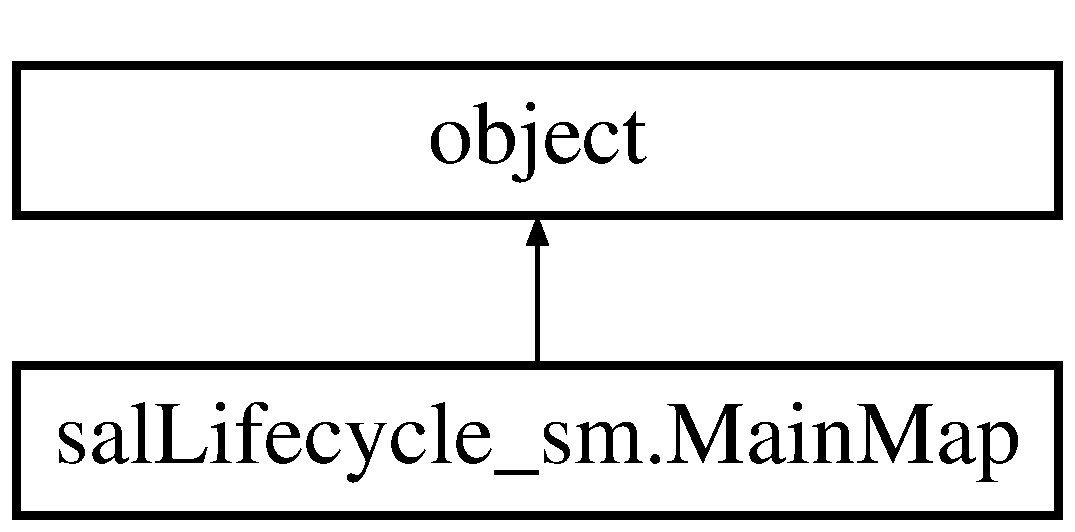
\includegraphics[height=2.000000cm]{classsal_lifecycle__sm_1_1_main_map}
\end{center}
\end{figure}
\subsection*{Static Public Attributes}
\begin{DoxyCompactItemize}
\item 
\hypertarget{classsal_lifecycle__sm_1_1_main_map_aa067cc6e61010a5e1420b1aac6a019f7}{tuple {\bfseries Off} = \hyperlink{classsal_lifecycle__sm_1_1_main_map___off}{Main\-Map\-\_\-\-Off}('Main\-Map.\-Off', 0)}\label{classsal_lifecycle__sm_1_1_main_map_aa067cc6e61010a5e1420b1aac6a019f7}

\item 
\hypertarget{classsal_lifecycle__sm_1_1_main_map_ad16f7e0b2bd7dbb80c39c130c7c633f5}{tuple {\bfseries S\-T\-A\-N\-D\-B\-Y} = \hyperlink{classsal_lifecycle__sm_1_1_main_map___s_t_a_n_d_b_y}{Main\-Map\-\_\-\-S\-T\-A\-N\-D\-B\-Y}('Main\-Map.\-S\-T\-A\-N\-D\-B\-Y', 1)}\label{classsal_lifecycle__sm_1_1_main_map_ad16f7e0b2bd7dbb80c39c130c7c633f5}

\item 
\hypertarget{classsal_lifecycle__sm_1_1_main_map_a1a4bf47c1b43c66a9a758a6f548eeccf}{tuple {\bfseries C\-O\-N\-F\-I\-G\-U\-R\-I\-N\-G} = \hyperlink{classsal_lifecycle__sm_1_1_main_map___c_o_n_f_i_g_u_r_i_n_g}{Main\-Map\-\_\-\-C\-O\-N\-F\-I\-G\-U\-R\-I\-N\-G}('Main\-Map.\-C\-O\-N\-F\-I\-G\-U\-R\-I\-N\-G', 2)}\label{classsal_lifecycle__sm_1_1_main_map_a1a4bf47c1b43c66a9a758a6f548eeccf}

\item 
\hypertarget{classsal_lifecycle__sm_1_1_main_map_af66acbd4e566b358d6d63839f16d338e}{tuple {\bfseries D\-I\-S\-A\-B\-L\-E\-D} = \hyperlink{classsal_lifecycle__sm_1_1_main_map___d_i_s_a_b_l_e_d}{Main\-Map\-\_\-\-D\-I\-S\-A\-B\-L\-E\-D}('Main\-Map.\-D\-I\-S\-A\-B\-L\-E\-D', 3)}\label{classsal_lifecycle__sm_1_1_main_map_af66acbd4e566b358d6d63839f16d338e}

\item 
\hypertarget{classsal_lifecycle__sm_1_1_main_map_a46fab8750ba572fd4e8fd592d56722ee}{tuple {\bfseries E\-N\-A\-B\-L\-E\-D} = \hyperlink{classsal_lifecycle__sm_1_1_main_map___e_n_a_b_l_e_d}{Main\-Map\-\_\-\-E\-N\-A\-B\-L\-E\-D}('Main\-Map.\-E\-N\-A\-B\-L\-E\-D', 4)}\label{classsal_lifecycle__sm_1_1_main_map_a46fab8750ba572fd4e8fd592d56722ee}

\item 
\hypertarget{classsal_lifecycle__sm_1_1_main_map_a999e17223acff64f2ec5d07aca40c373}{tuple {\bfseries E\-R\-R\-O\-R} = \hyperlink{classsal_lifecycle__sm_1_1_main_map___e_r_r_o_r}{Main\-Map\-\_\-\-E\-R\-R\-O\-R}('Main\-Map.\-E\-R\-R\-O\-R', 5)}\label{classsal_lifecycle__sm_1_1_main_map_a999e17223acff64f2ec5d07aca40c373}

\item 
\hypertarget{classsal_lifecycle__sm_1_1_main_map_a27cccc860bf1654f3fc282be9eff2a88}{tuple {\bfseries Default} = \hyperlink{classsal_lifecycle__sm_1_1_main_map___default}{Main\-Map\-\_\-\-Default}('Main\-Map.\-Default', -\/1)}\label{classsal_lifecycle__sm_1_1_main_map_a27cccc860bf1654f3fc282be9eff2a88}

\end{DoxyCompactItemize}


\subsection{Detailed Description}


Definition at line 239 of file sal\-Lifecycle\-\_\-sm.\-py.



The documentation for this class was generated from the following file\-:\begin{DoxyCompactItemize}
\item 
/opt/lsstsal/state\-Machine/python/sal\-Lifecycle\-\_\-sm.\-py\end{DoxyCompactItemize}

\hypertarget{class_main_map___c_o_n_f_i_g_u_r_i_n_g}{\section{Main\-Map\-\_\-\-C\-O\-N\-F\-I\-G\-U\-R\-I\-N\-G Class Reference}
\label{class_main_map___c_o_n_f_i_g_u_r_i_n_g}\index{Main\-Map\-\_\-\-C\-O\-N\-F\-I\-G\-U\-R\-I\-N\-G@{Main\-Map\-\_\-\-C\-O\-N\-F\-I\-G\-U\-R\-I\-N\-G}}
}
Inheritance diagram for Main\-Map\-\_\-\-C\-O\-N\-F\-I\-G\-U\-R\-I\-N\-G\-:\begin{figure}[H]
\begin{center}
\leavevmode
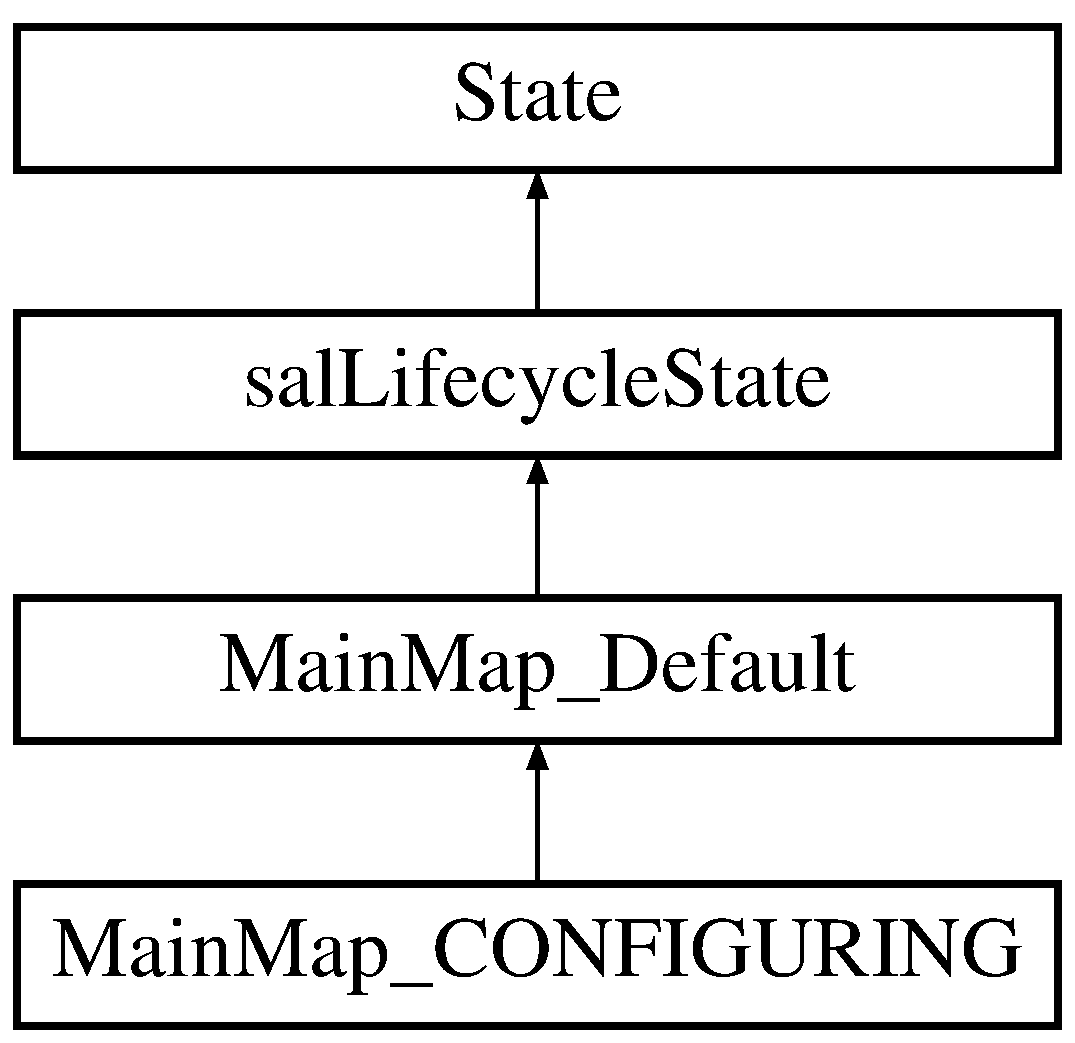
\includegraphics[height=4.000000cm]{class_main_map___c_o_n_f_i_g_u_r_i_n_g}
\end{center}
\end{figure}
\subsection*{Public Member Functions}
\begin{DoxyCompactItemize}
\item 
\hypertarget{class_main_map___c_o_n_f_i_g_u_r_i_n_g_a4a628ef377e47019ab7b03b243fc304e}{{\bfseries Main\-Map\-\_\-\-C\-O\-N\-F\-I\-G\-U\-R\-I\-N\-G} (const char $\ast$const name, const int state\-Id)}\label{class_main_map___c_o_n_f_i_g_u_r_i_n_g_a4a628ef377e47019ab7b03b243fc304e}

\item 
\hypertarget{class_main_map___c_o_n_f_i_g_u_r_i_n_g_a6858f68400aed8f12d65489f2698515c}{virtual void {\bfseries configure\-Error} (sal\-Lifecycle-\/\hyperlink{classcpp_context}{cpp\-Context} \&context)}\label{class_main_map___c_o_n_f_i_g_u_r_i_n_g_a6858f68400aed8f12d65489f2698515c}

\item 
\hypertarget{class_main_map___c_o_n_f_i_g_u_r_i_n_g_afd15e4e4a800ab7cd8a7a74756da9e7d}{virtual void {\bfseries ocs\-Abandon} (sal\-Lifecycle-\/\hyperlink{classcpp_context}{cpp\-Context} \&context)}\label{class_main_map___c_o_n_f_i_g_u_r_i_n_g_afd15e4e4a800ab7cd8a7a74756da9e7d}

\item 
\hypertarget{class_main_map___c_o_n_f_i_g_u_r_i_n_g_a3978d4b67799d01afd12740000e25d99}{virtual void {\bfseries ocs\-Configure} (sal\-Lifecycle-\/\hyperlink{classcpp_context}{cpp\-Context} \&context)}\label{class_main_map___c_o_n_f_i_g_u_r_i_n_g_a3978d4b67799d01afd12740000e25d99}

\end{DoxyCompactItemize}
\subsection*{Additional Inherited Members}


\subsection{Detailed Description}


Definition at line 107 of file sal\-Lifecycle-\/cpp\-\_\-sm.\-h.



The documentation for this class was generated from the following files\-:\begin{DoxyCompactItemize}
\item 
/opt/lsstsal/state\-Machine/cpp/sal\-Lifecycle-\/cpp\-\_\-sm.\-h\item 
/opt/lsstsal/state\-Machine/cpp/sal\-Lifecycle-\/cpp\-\_\-sm.\-cpp\end{DoxyCompactItemize}

\hypertarget{classsal_lifecycle__sm_1_1_main_map___c_o_n_f_i_g_u_r_i_n_g}{\section{sal\-Lifecycle\-\_\-sm.\-Main\-Map\-\_\-\-C\-O\-N\-F\-I\-G\-U\-R\-I\-N\-G Class Reference}
\label{classsal_lifecycle__sm_1_1_main_map___c_o_n_f_i_g_u_r_i_n_g}\index{sal\-Lifecycle\-\_\-sm.\-Main\-Map\-\_\-\-C\-O\-N\-F\-I\-G\-U\-R\-I\-N\-G@{sal\-Lifecycle\-\_\-sm.\-Main\-Map\-\_\-\-C\-O\-N\-F\-I\-G\-U\-R\-I\-N\-G}}
}
Inheritance diagram for sal\-Lifecycle\-\_\-sm.\-Main\-Map\-\_\-\-C\-O\-N\-F\-I\-G\-U\-R\-I\-N\-G\-:\begin{figure}[H]
\begin{center}
\leavevmode
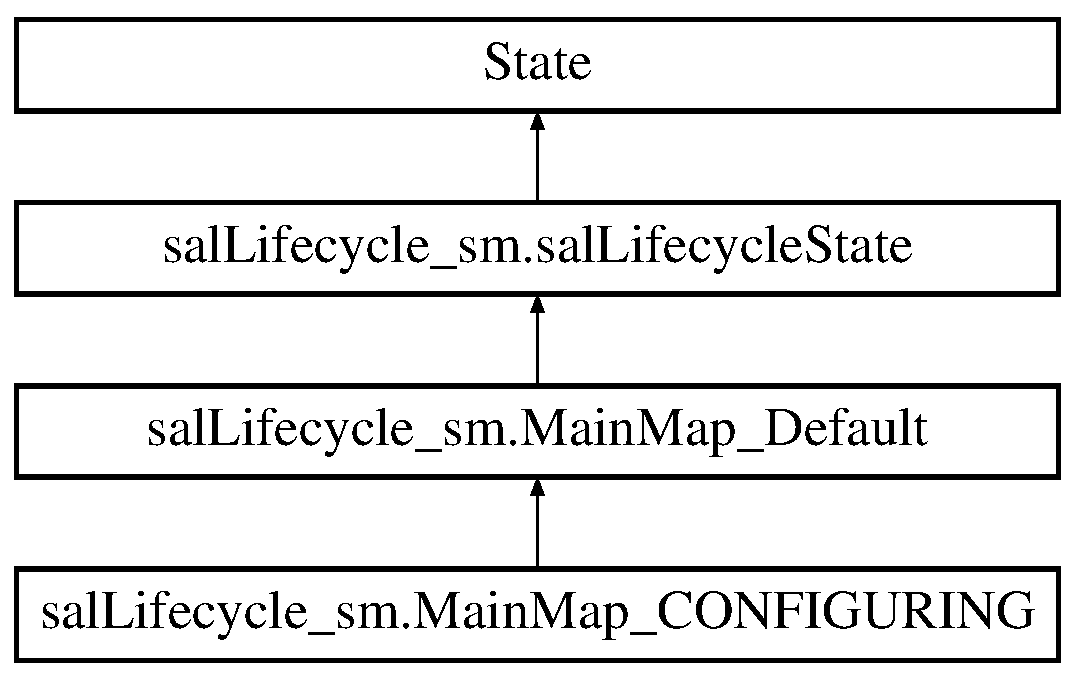
\includegraphics[height=4.000000cm]{classsal_lifecycle__sm_1_1_main_map___c_o_n_f_i_g_u_r_i_n_g}
\end{center}
\end{figure}
\subsection*{Public Member Functions}
\begin{DoxyCompactItemize}
\item 
\hypertarget{classsal_lifecycle__sm_1_1_main_map___c_o_n_f_i_g_u_r_i_n_g_a2c13841d2bc1e4791b75bf3c93638d8d}{def {\bfseries configure\-Error}}\label{classsal_lifecycle__sm_1_1_main_map___c_o_n_f_i_g_u_r_i_n_g_a2c13841d2bc1e4791b75bf3c93638d8d}

\item 
\hypertarget{classsal_lifecycle__sm_1_1_main_map___c_o_n_f_i_g_u_r_i_n_g_a8e52976b6a56f8282c415c89e9e1d940}{def {\bfseries ocs\-Abandon}}\label{classsal_lifecycle__sm_1_1_main_map___c_o_n_f_i_g_u_r_i_n_g_a8e52976b6a56f8282c415c89e9e1d940}

\item 
\hypertarget{classsal_lifecycle__sm_1_1_main_map___c_o_n_f_i_g_u_r_i_n_g_af61b61dd4536f1cec2c89a2b59263efa}{def {\bfseries ocs\-Configure}}\label{classsal_lifecycle__sm_1_1_main_map___c_o_n_f_i_g_u_r_i_n_g_af61b61dd4536f1cec2c89a2b59263efa}

\end{DoxyCompactItemize}


\subsection{Detailed Description}


Definition at line 101 of file sal\-Lifecycle\-\_\-sm.\-py.



The documentation for this class was generated from the following file\-:\begin{DoxyCompactItemize}
\item 
/opt/lsstsal/state\-Machine/python/sal\-Lifecycle\-\_\-sm.\-py\end{DoxyCompactItemize}

\hypertarget{classsal_lifecycle__sm_1_1_main_map___default}{\section{sal\-Lifecycle\-\_\-sm.\-Main\-Map\-\_\-\-Default Class Reference}
\label{classsal_lifecycle__sm_1_1_main_map___default}\index{sal\-Lifecycle\-\_\-sm.\-Main\-Map\-\_\-\-Default@{sal\-Lifecycle\-\_\-sm.\-Main\-Map\-\_\-\-Default}}
}
Inheritance diagram for sal\-Lifecycle\-\_\-sm.\-Main\-Map\-\_\-\-Default\-:\begin{figure}[H]
\begin{center}
\leavevmode
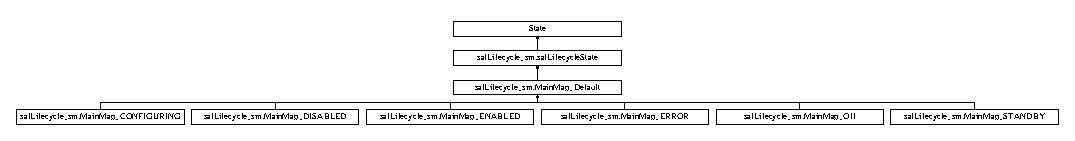
\includegraphics[height=1.441441cm]{classsal_lifecycle__sm_1_1_main_map___default}
\end{center}
\end{figure}
\subsection*{Additional Inherited Members}


\subsection{Detailed Description}


Definition at line 64 of file sal\-Lifecycle\-\_\-sm.\-py.



The documentation for this class was generated from the following file\-:\begin{DoxyCompactItemize}
\item 
/opt/lsstsal/state\-Machine/python/sal\-Lifecycle\-\_\-sm.\-py\end{DoxyCompactItemize}

\hypertarget{class_main_map___default}{\section{Main\-Map\-\_\-\-Default Class Reference}
\label{class_main_map___default}\index{Main\-Map\-\_\-\-Default@{Main\-Map\-\_\-\-Default}}
}
Inheritance diagram for Main\-Map\-\_\-\-Default\-:\begin{figure}[H]
\begin{center}
\leavevmode
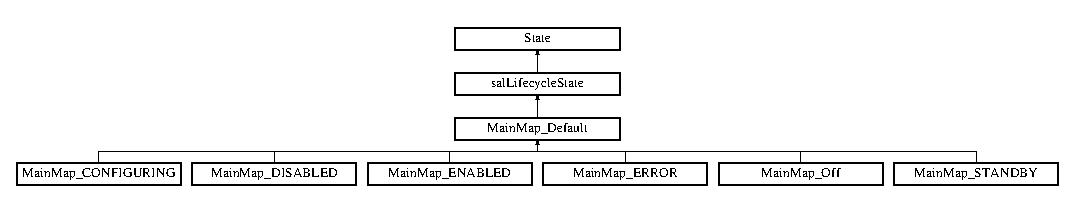
\includegraphics[height=2.262626cm]{class_main_map___default}
\end{center}
\end{figure}
\subsection*{Public Member Functions}
\begin{DoxyCompactItemize}
\item 
\hypertarget{class_main_map___default_a61e352bbc45058065a51410e7c9f5f1f}{{\bfseries Main\-Map\-\_\-\-Default} (const char $\ast$const name, const int state\-Id)}\label{class_main_map___default_a61e352bbc45058065a51410e7c9f5f1f}

\end{DoxyCompactItemize}
\subsection*{Additional Inherited Members}


\subsection{Detailed Description}


Definition at line 73 of file sal\-Lifecycle-\/cpp\-\_\-sm.\-h.



The documentation for this class was generated from the following file\-:\begin{DoxyCompactItemize}
\item 
/opt/lsstsal/state\-Machine/cpp/sal\-Lifecycle-\/cpp\-\_\-sm.\-h\end{DoxyCompactItemize}

\hypertarget{classsal_lifecycle__sm_1_1_main_map___d_i_s_a_b_l_e_d}{\section{sal\-Lifecycle\-\_\-sm.\-Main\-Map\-\_\-\-D\-I\-S\-A\-B\-L\-E\-D Class Reference}
\label{classsal_lifecycle__sm_1_1_main_map___d_i_s_a_b_l_e_d}\index{sal\-Lifecycle\-\_\-sm.\-Main\-Map\-\_\-\-D\-I\-S\-A\-B\-L\-E\-D@{sal\-Lifecycle\-\_\-sm.\-Main\-Map\-\_\-\-D\-I\-S\-A\-B\-L\-E\-D}}
}
Inheritance diagram for sal\-Lifecycle\-\_\-sm.\-Main\-Map\-\_\-\-D\-I\-S\-A\-B\-L\-E\-D\-:\begin{figure}[H]
\begin{center}
\leavevmode
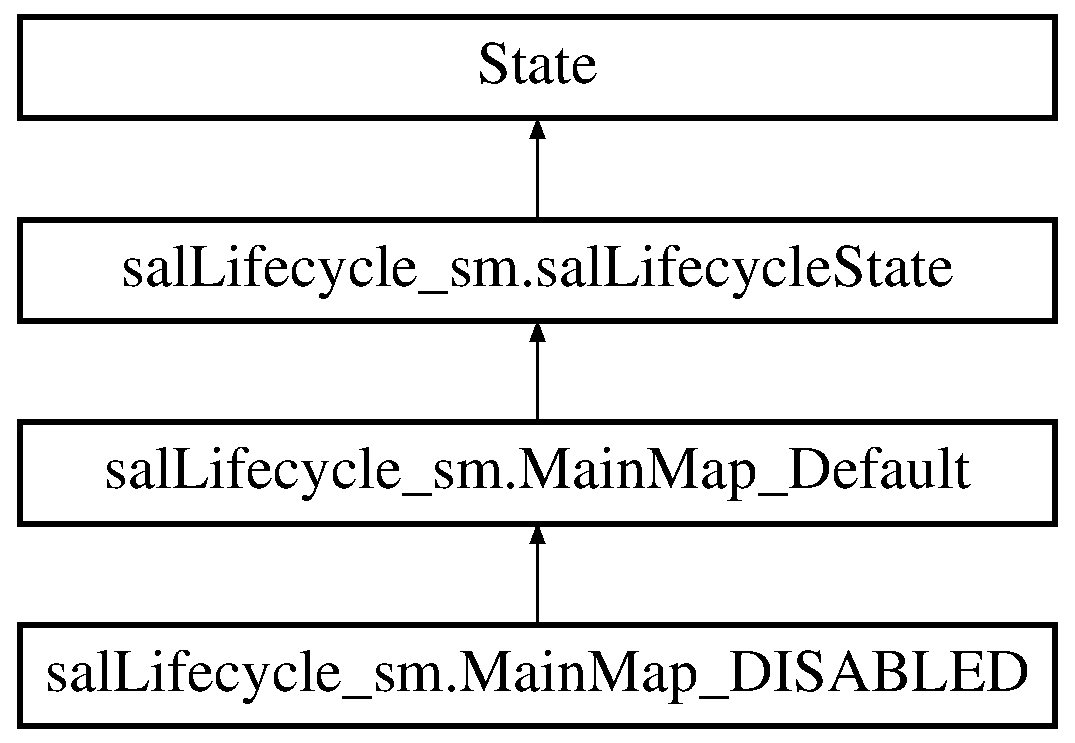
\includegraphics[height=4.000000cm]{classsal_lifecycle__sm_1_1_main_map___d_i_s_a_b_l_e_d}
\end{center}
\end{figure}
\subsection*{Public Member Functions}
\begin{DoxyCompactItemize}
\item 
\hypertarget{classsal_lifecycle__sm_1_1_main_map___d_i_s_a_b_l_e_d_ad0e8ccfa8b3903201e6fb7d44a75a0a5}{def {\bfseries disable\-Error}}\label{classsal_lifecycle__sm_1_1_main_map___d_i_s_a_b_l_e_d_ad0e8ccfa8b3903201e6fb7d44a75a0a5}

\item 
\hypertarget{classsal_lifecycle__sm_1_1_main_map___d_i_s_a_b_l_e_d_a409afd12f8ff1f41557006b2f075f169}{def {\bfseries ocs\-Enable}}\label{classsal_lifecycle__sm_1_1_main_map___d_i_s_a_b_l_e_d_a409afd12f8ff1f41557006b2f075f169}

\item 
\hypertarget{classsal_lifecycle__sm_1_1_main_map___d_i_s_a_b_l_e_d_aecdf17bcbb1d82ae934ffab92f8c62f0}{def {\bfseries ocs\-Un\-Configure}}\label{classsal_lifecycle__sm_1_1_main_map___d_i_s_a_b_l_e_d_aecdf17bcbb1d82ae934ffab92f8c62f0}

\end{DoxyCompactItemize}


\subsection{Detailed Description}


Definition at line 133 of file sal\-Lifecycle\-\_\-sm.\-py.



The documentation for this class was generated from the following file\-:\begin{DoxyCompactItemize}
\item 
/opt/lsstsal/state\-Machine/python/sal\-Lifecycle\-\_\-sm.\-py\end{DoxyCompactItemize}

\hypertarget{class_main_map___d_i_s_a_b_l_e_d}{\section{Main\-Map\-\_\-\-D\-I\-S\-A\-B\-L\-E\-D Class Reference}
\label{class_main_map___d_i_s_a_b_l_e_d}\index{Main\-Map\-\_\-\-D\-I\-S\-A\-B\-L\-E\-D@{Main\-Map\-\_\-\-D\-I\-S\-A\-B\-L\-E\-D}}
}
Inheritance diagram for Main\-Map\-\_\-\-D\-I\-S\-A\-B\-L\-E\-D\-:\begin{figure}[H]
\begin{center}
\leavevmode
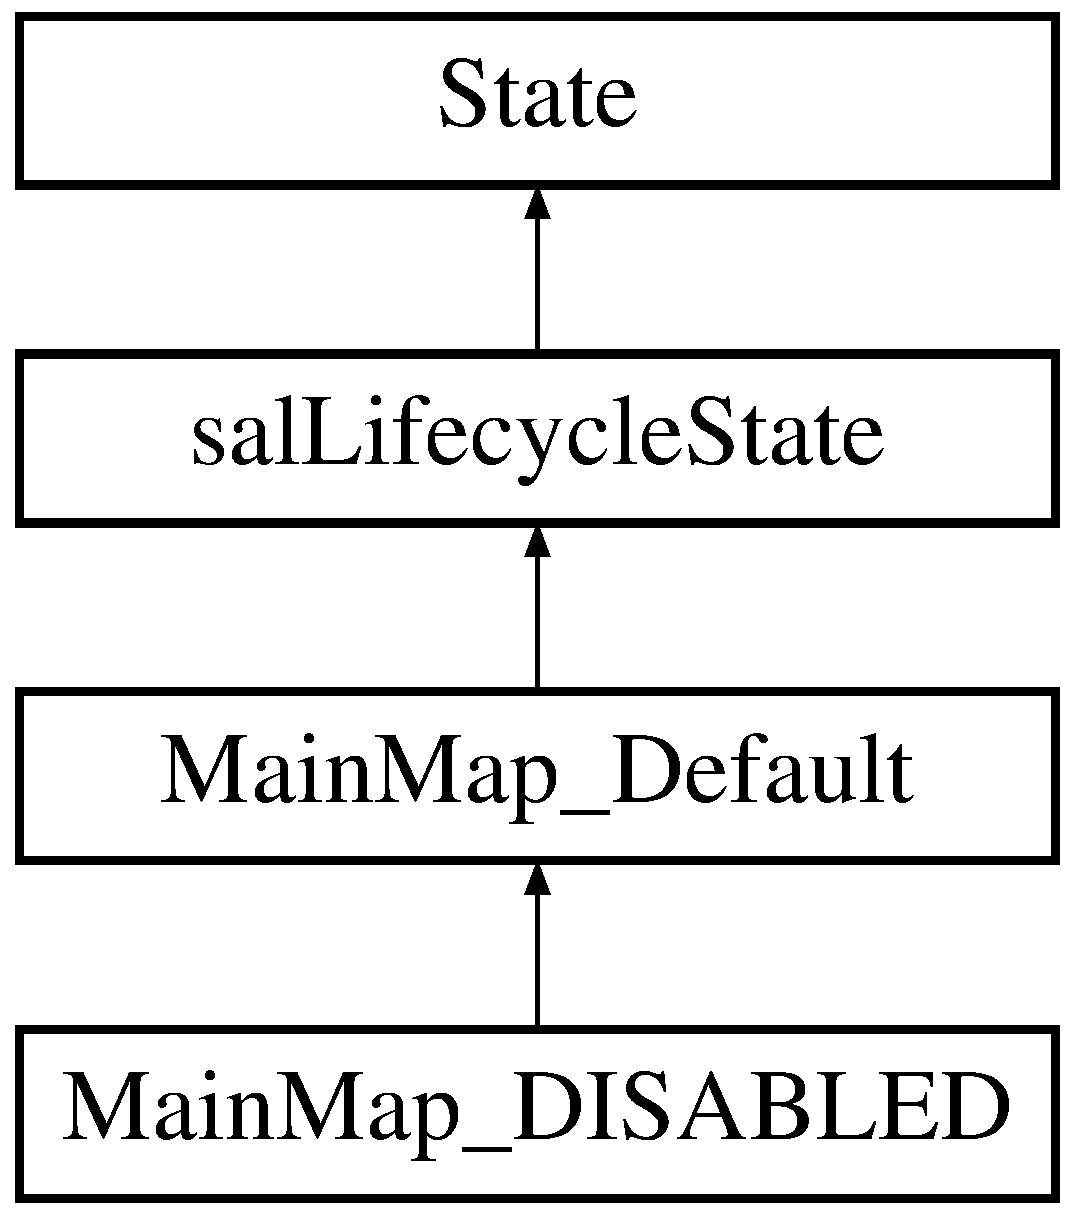
\includegraphics[height=4.000000cm]{class_main_map___d_i_s_a_b_l_e_d}
\end{center}
\end{figure}
\subsection*{Public Member Functions}
\begin{DoxyCompactItemize}
\item 
\hypertarget{class_main_map___d_i_s_a_b_l_e_d_aed634fa3479d60f76a353baf601560d5}{{\bfseries Main\-Map\-\_\-\-D\-I\-S\-A\-B\-L\-E\-D} (const char $\ast$const name, const int state\-Id)}\label{class_main_map___d_i_s_a_b_l_e_d_aed634fa3479d60f76a353baf601560d5}

\item 
\hypertarget{class_main_map___d_i_s_a_b_l_e_d_a47d98da0abb45f3fdfabf1cfcff7975a}{virtual void {\bfseries disable\-Error} (sal\-Lifecycle-\/\hyperlink{classcpp_context}{cpp\-Context} \&context)}\label{class_main_map___d_i_s_a_b_l_e_d_a47d98da0abb45f3fdfabf1cfcff7975a}

\item 
\hypertarget{class_main_map___d_i_s_a_b_l_e_d_aa49b5cdd59dc9c575a55c8ea9ee5ba3e}{virtual void {\bfseries ocs\-Enable} (sal\-Lifecycle-\/\hyperlink{classcpp_context}{cpp\-Context} \&context)}\label{class_main_map___d_i_s_a_b_l_e_d_aa49b5cdd59dc9c575a55c8ea9ee5ba3e}

\item 
\hypertarget{class_main_map___d_i_s_a_b_l_e_d_a401fa73a5d80d332e460dde2cbd00393}{virtual void {\bfseries ocs\-Un\-Configure} (sal\-Lifecycle-\/\hyperlink{classcpp_context}{cpp\-Context} \&context)}\label{class_main_map___d_i_s_a_b_l_e_d_a401fa73a5d80d332e460dde2cbd00393}

\end{DoxyCompactItemize}
\subsection*{Additional Inherited Members}


\subsection{Detailed Description}


Definition at line 120 of file sal\-Lifecycle-\/cpp\-\_\-sm.\-h.



The documentation for this class was generated from the following files\-:\begin{DoxyCompactItemize}
\item 
/opt/lsstsal/state\-Machine/cpp/sal\-Lifecycle-\/cpp\-\_\-sm.\-h\item 
/opt/lsstsal/state\-Machine/cpp/sal\-Lifecycle-\/cpp\-\_\-sm.\-cpp\end{DoxyCompactItemize}

\hypertarget{class_main_map___e_n_a_b_l_e_d}{\section{Main\-Map\-\_\-\-E\-N\-A\-B\-L\-E\-D Class Reference}
\label{class_main_map___e_n_a_b_l_e_d}\index{Main\-Map\-\_\-\-E\-N\-A\-B\-L\-E\-D@{Main\-Map\-\_\-\-E\-N\-A\-B\-L\-E\-D}}
}
Inheritance diagram for Main\-Map\-\_\-\-E\-N\-A\-B\-L\-E\-D\-:\begin{figure}[H]
\begin{center}
\leavevmode
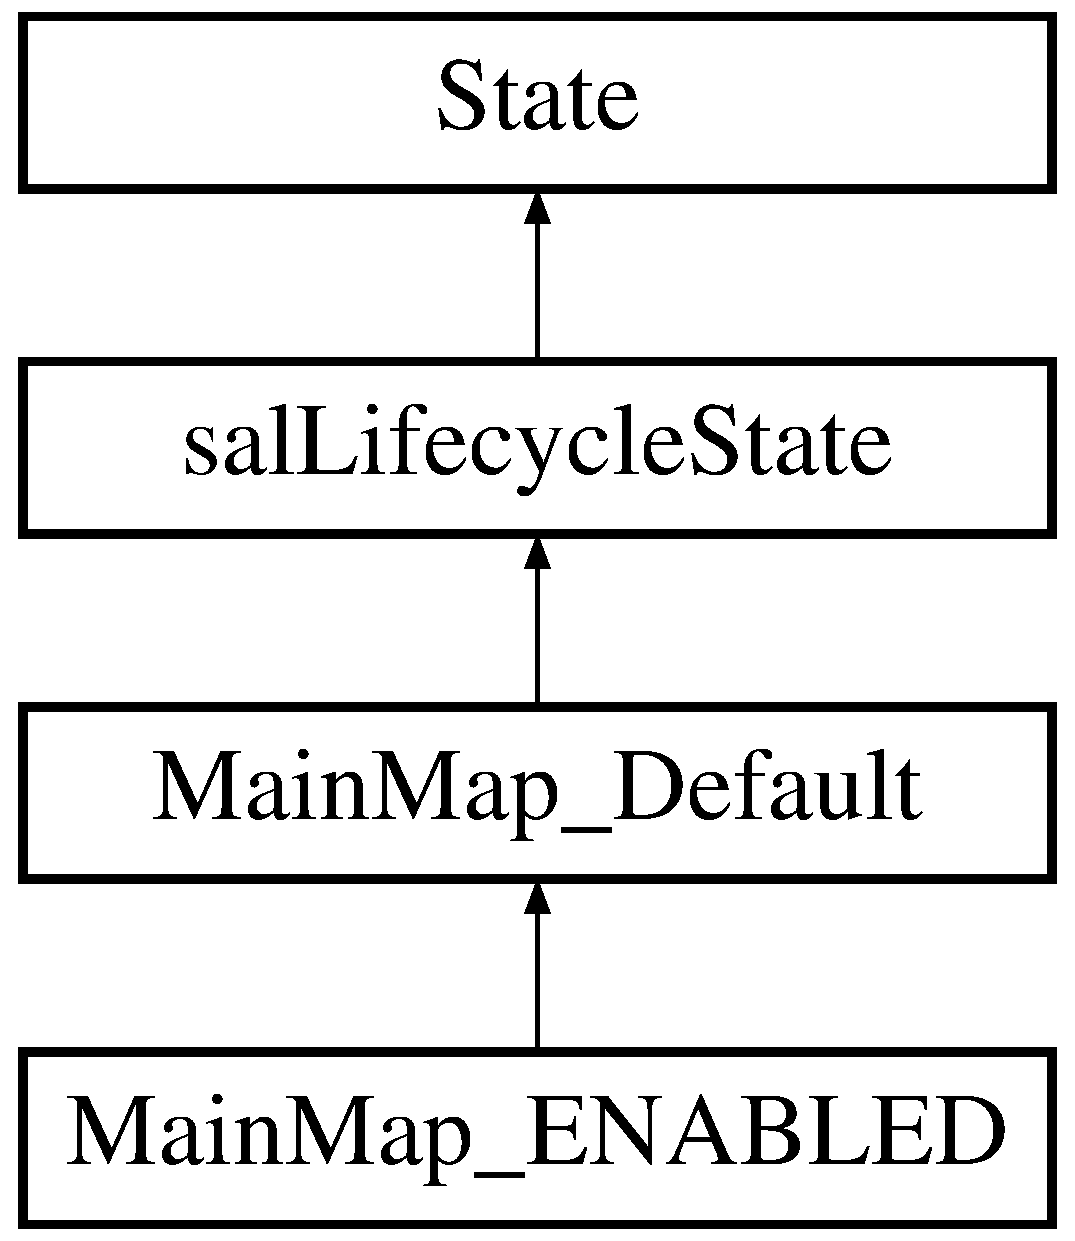
\includegraphics[height=4.000000cm]{class_main_map___e_n_a_b_l_e_d}
\end{center}
\end{figure}
\subsection*{Public Member Functions}
\begin{DoxyCompactItemize}
\item 
\hypertarget{class_main_map___e_n_a_b_l_e_d_ad3a00ff99ae36f1d094c4562e0e30497}{{\bfseries Main\-Map\-\_\-\-E\-N\-A\-B\-L\-E\-D} (const char $\ast$const name, const int state\-Id)}\label{class_main_map___e_n_a_b_l_e_d_ad3a00ff99ae36f1d094c4562e0e30497}

\item 
\hypertarget{class_main_map___e_n_a_b_l_e_d_a2cf5603cef40ed302f02e48e08c4a4f3}{virtual void {\bfseries enable\-Error} (sal\-Lifecycle-\/\hyperlink{classcpp_context}{cpp\-Context} \&context)}\label{class_main_map___e_n_a_b_l_e_d_a2cf5603cef40ed302f02e48e08c4a4f3}

\item 
\hypertarget{class_main_map___e_n_a_b_l_e_d_a55b1bd24594fb648a0283dde42bbb9da}{virtual void {\bfseries ocs\-Abort} (sal\-Lifecycle-\/\hyperlink{classcpp_context}{cpp\-Context} \&context)}\label{class_main_map___e_n_a_b_l_e_d_a55b1bd24594fb648a0283dde42bbb9da}

\item 
\hypertarget{class_main_map___e_n_a_b_l_e_d_aed12076f2daa8f7ed4aba7b290781584}{virtual void {\bfseries ocs\-Disable} (sal\-Lifecycle-\/\hyperlink{classcpp_context}{cpp\-Context} \&context)}\label{class_main_map___e_n_a_b_l_e_d_aed12076f2daa8f7ed4aba7b290781584}

\item 
\hypertarget{class_main_map___e_n_a_b_l_e_d_a0775a62bde51b04b71fa60eef9a67b2e}{virtual void {\bfseries ocs\-Enable} (sal\-Lifecycle-\/\hyperlink{classcpp_context}{cpp\-Context} \&context)}\label{class_main_map___e_n_a_b_l_e_d_a0775a62bde51b04b71fa60eef9a67b2e}

\item 
\hypertarget{class_main_map___e_n_a_b_l_e_d_ac4c7a82a404b1fd3b7b394f11b7dfeee}{virtual void {\bfseries ocs\-Set\-Value} (sal\-Lifecycle-\/\hyperlink{classcpp_context}{cpp\-Context} \&context)}\label{class_main_map___e_n_a_b_l_e_d_ac4c7a82a404b1fd3b7b394f11b7dfeee}

\item 
\hypertarget{class_main_map___e_n_a_b_l_e_d_afe087f68d6aa7402a7198b67f0b2b1e5}{virtual void {\bfseries ocs\-Stop} (sal\-Lifecycle-\/\hyperlink{classcpp_context}{cpp\-Context} \&context)}\label{class_main_map___e_n_a_b_l_e_d_afe087f68d6aa7402a7198b67f0b2b1e5}

\end{DoxyCompactItemize}
\subsection*{Additional Inherited Members}


\subsection{Detailed Description}


Definition at line 133 of file sal\-Lifecycle-\/cpp\-\_\-sm.\-h.



The documentation for this class was generated from the following files\-:\begin{DoxyCompactItemize}
\item 
/opt/lsstsal/state\-Machine/cpp/sal\-Lifecycle-\/cpp\-\_\-sm.\-h\item 
/opt/lsstsal/state\-Machine/cpp/sal\-Lifecycle-\/cpp\-\_\-sm.\-cpp\end{DoxyCompactItemize}

\hypertarget{classsal_lifecycle__sm_1_1_main_map___e_n_a_b_l_e_d}{\section{sal\-Lifecycle\-\_\-sm.\-Main\-Map\-\_\-\-E\-N\-A\-B\-L\-E\-D Class Reference}
\label{classsal_lifecycle__sm_1_1_main_map___e_n_a_b_l_e_d}\index{sal\-Lifecycle\-\_\-sm.\-Main\-Map\-\_\-\-E\-N\-A\-B\-L\-E\-D@{sal\-Lifecycle\-\_\-sm.\-Main\-Map\-\_\-\-E\-N\-A\-B\-L\-E\-D}}
}
Inheritance diagram for sal\-Lifecycle\-\_\-sm.\-Main\-Map\-\_\-\-E\-N\-A\-B\-L\-E\-D\-:\begin{figure}[H]
\begin{center}
\leavevmode
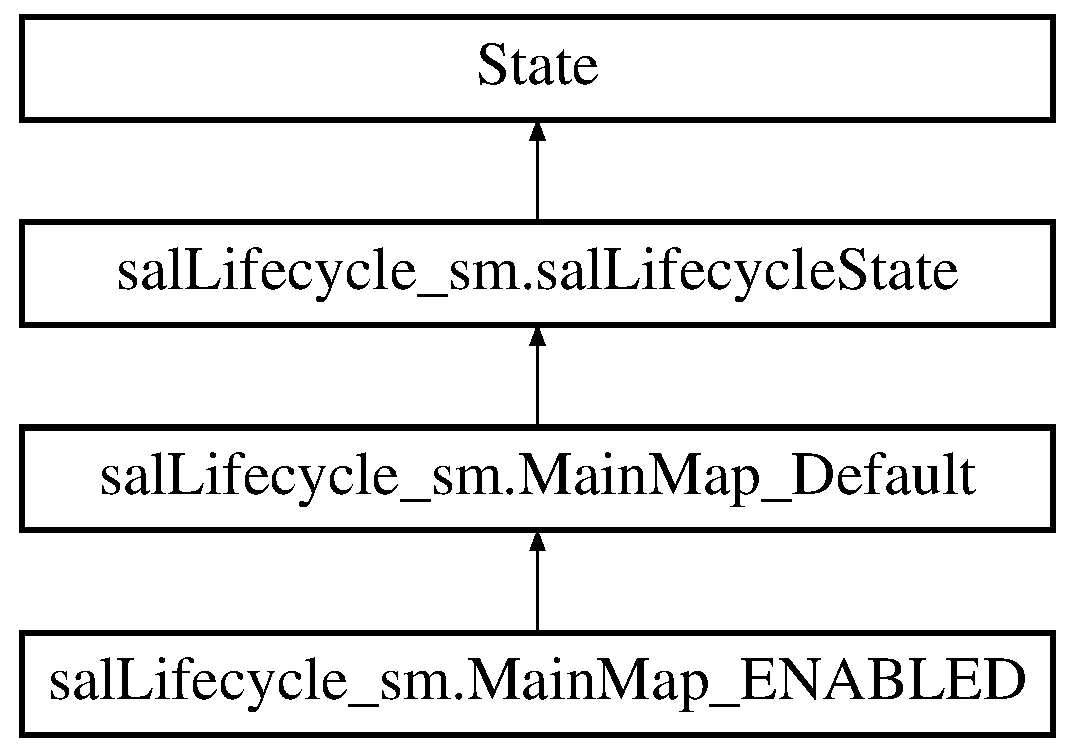
\includegraphics[height=4.000000cm]{classsal_lifecycle__sm_1_1_main_map___e_n_a_b_l_e_d}
\end{center}
\end{figure}
\subsection*{Public Member Functions}
\begin{DoxyCompactItemize}
\item 
\hypertarget{classsal_lifecycle__sm_1_1_main_map___e_n_a_b_l_e_d_a142b9d53b23056fe1cdb4acb67c1f6bd}{def {\bfseries enable\-Error}}\label{classsal_lifecycle__sm_1_1_main_map___e_n_a_b_l_e_d_a142b9d53b23056fe1cdb4acb67c1f6bd}

\item 
\hypertarget{classsal_lifecycle__sm_1_1_main_map___e_n_a_b_l_e_d_ab0717532028be7ef92c47d7c1f67eb90}{def {\bfseries ocs\-Abort}}\label{classsal_lifecycle__sm_1_1_main_map___e_n_a_b_l_e_d_ab0717532028be7ef92c47d7c1f67eb90}

\item 
\hypertarget{classsal_lifecycle__sm_1_1_main_map___e_n_a_b_l_e_d_a4ad6c9393a013cbab8c1298d5c7b90c1}{def {\bfseries ocs\-Disable}}\label{classsal_lifecycle__sm_1_1_main_map___e_n_a_b_l_e_d_a4ad6c9393a013cbab8c1298d5c7b90c1}

\item 
\hypertarget{classsal_lifecycle__sm_1_1_main_map___e_n_a_b_l_e_d_af6f545b868e009472823d2801a18ef50}{def {\bfseries ocs\-Enable}}\label{classsal_lifecycle__sm_1_1_main_map___e_n_a_b_l_e_d_af6f545b868e009472823d2801a18ef50}

\item 
\hypertarget{classsal_lifecycle__sm_1_1_main_map___e_n_a_b_l_e_d_a29e538873ec8e57e5d75d88220df50fd}{def {\bfseries ocs\-Set\-Value}}\label{classsal_lifecycle__sm_1_1_main_map___e_n_a_b_l_e_d_a29e538873ec8e57e5d75d88220df50fd}

\item 
\hypertarget{classsal_lifecycle__sm_1_1_main_map___e_n_a_b_l_e_d_ab9920fcdc9c284a019c27ed01d0a9d29}{def {\bfseries ocs\-Stop}}\label{classsal_lifecycle__sm_1_1_main_map___e_n_a_b_l_e_d_ab9920fcdc9c284a019c27ed01d0a9d29}

\end{DoxyCompactItemize}


\subsection{Detailed Description}


Definition at line 165 of file sal\-Lifecycle\-\_\-sm.\-py.



The documentation for this class was generated from the following file\-:\begin{DoxyCompactItemize}
\item 
/opt/lsstsal/state\-Machine/python/sal\-Lifecycle\-\_\-sm.\-py\end{DoxyCompactItemize}

\hypertarget{class_main_map___e_r_r_o_r}{\section{Main\-Map\-\_\-\-E\-R\-R\-O\-R Class Reference}
\label{class_main_map___e_r_r_o_r}\index{Main\-Map\-\_\-\-E\-R\-R\-O\-R@{Main\-Map\-\_\-\-E\-R\-R\-O\-R}}
}
Inheritance diagram for Main\-Map\-\_\-\-E\-R\-R\-O\-R\-:\begin{figure}[H]
\begin{center}
\leavevmode
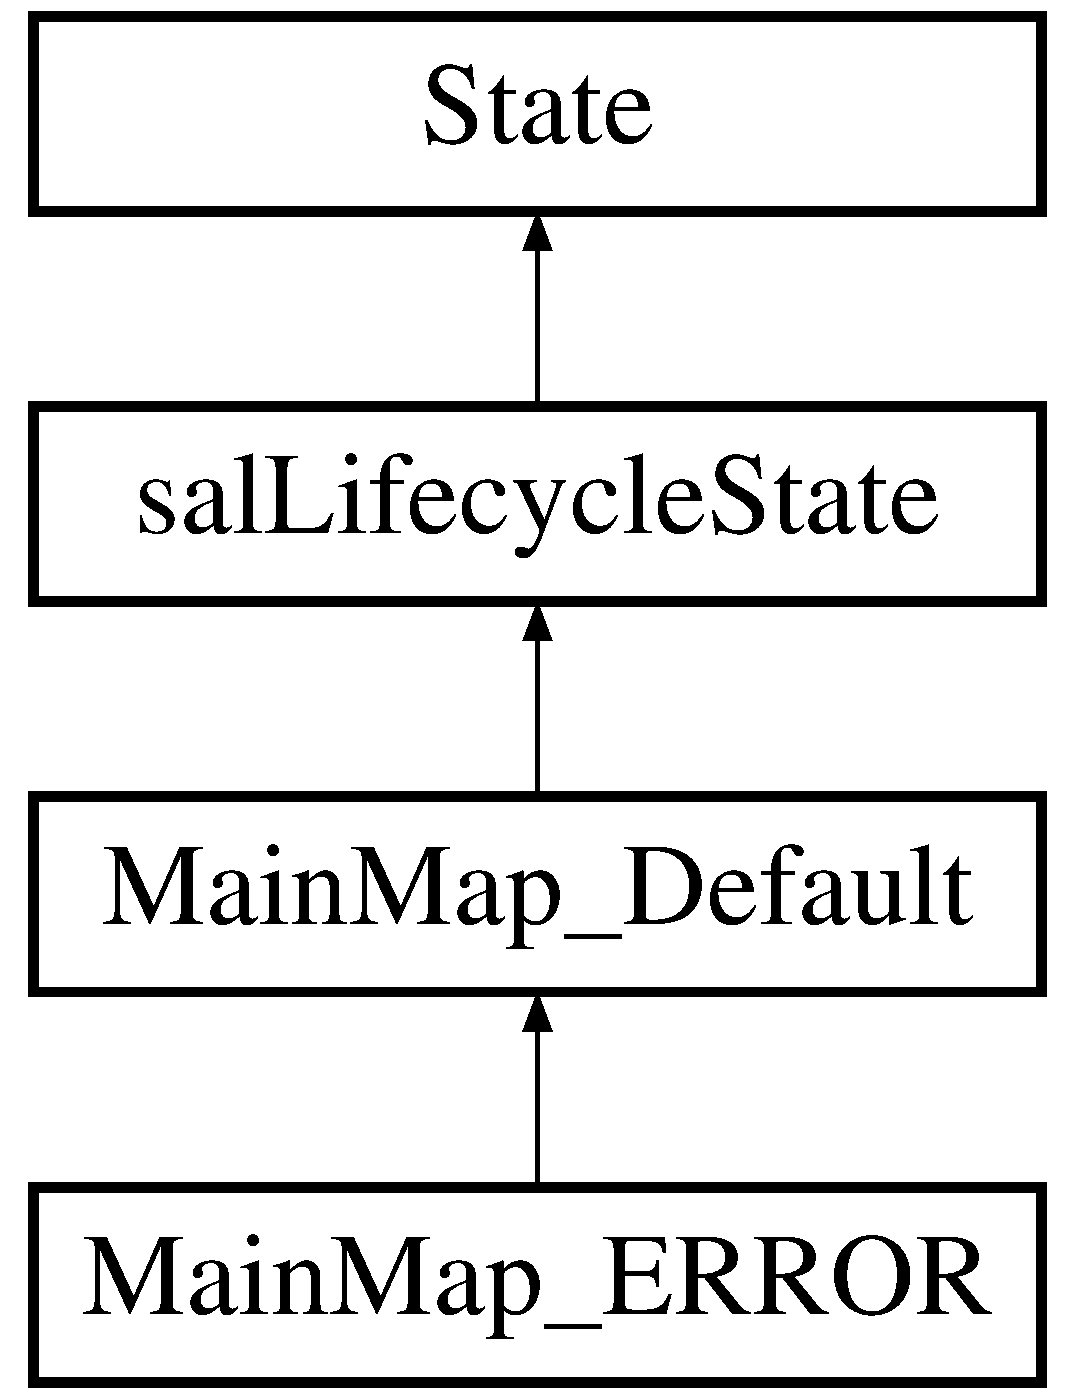
\includegraphics[height=4.000000cm]{class_main_map___e_r_r_o_r}
\end{center}
\end{figure}
\subsection*{Public Member Functions}
\begin{DoxyCompactItemize}
\item 
\hypertarget{class_main_map___e_r_r_o_r_ae06ea6dbe1d8f12eb91736baea016059}{{\bfseries Main\-Map\-\_\-\-E\-R\-R\-O\-R} (const char $\ast$const name, const int state\-Id)}\label{class_main_map___e_r_r_o_r_ae06ea6dbe1d8f12eb91736baea016059}

\item 
\hypertarget{class_main_map___e_r_r_o_r_ae6def65b95ff514701b13cd24eefa8d3}{virtual void {\bfseries ocs\-Reset} (sal\-Lifecycle-\/\hyperlink{classcpp_context}{cpp\-Context} \&context)}\label{class_main_map___e_r_r_o_r_ae6def65b95ff514701b13cd24eefa8d3}

\end{DoxyCompactItemize}
\subsection*{Additional Inherited Members}


\subsection{Detailed Description}


Definition at line 149 of file sal\-Lifecycle-\/cpp\-\_\-sm.\-h.



The documentation for this class was generated from the following files\-:\begin{DoxyCompactItemize}
\item 
/opt/lsstsal/state\-Machine/cpp/sal\-Lifecycle-\/cpp\-\_\-sm.\-h\item 
/opt/lsstsal/state\-Machine/cpp/sal\-Lifecycle-\/cpp\-\_\-sm.\-cpp\end{DoxyCompactItemize}

\hypertarget{classsal_lifecycle__sm_1_1_main_map___e_r_r_o_r}{\section{sal\-Lifecycle\-\_\-sm.\-Main\-Map\-\_\-\-E\-R\-R\-O\-R Class Reference}
\label{classsal_lifecycle__sm_1_1_main_map___e_r_r_o_r}\index{sal\-Lifecycle\-\_\-sm.\-Main\-Map\-\_\-\-E\-R\-R\-O\-R@{sal\-Lifecycle\-\_\-sm.\-Main\-Map\-\_\-\-E\-R\-R\-O\-R}}
}
Inheritance diagram for sal\-Lifecycle\-\_\-sm.\-Main\-Map\-\_\-\-E\-R\-R\-O\-R\-:\begin{figure}[H]
\begin{center}
\leavevmode
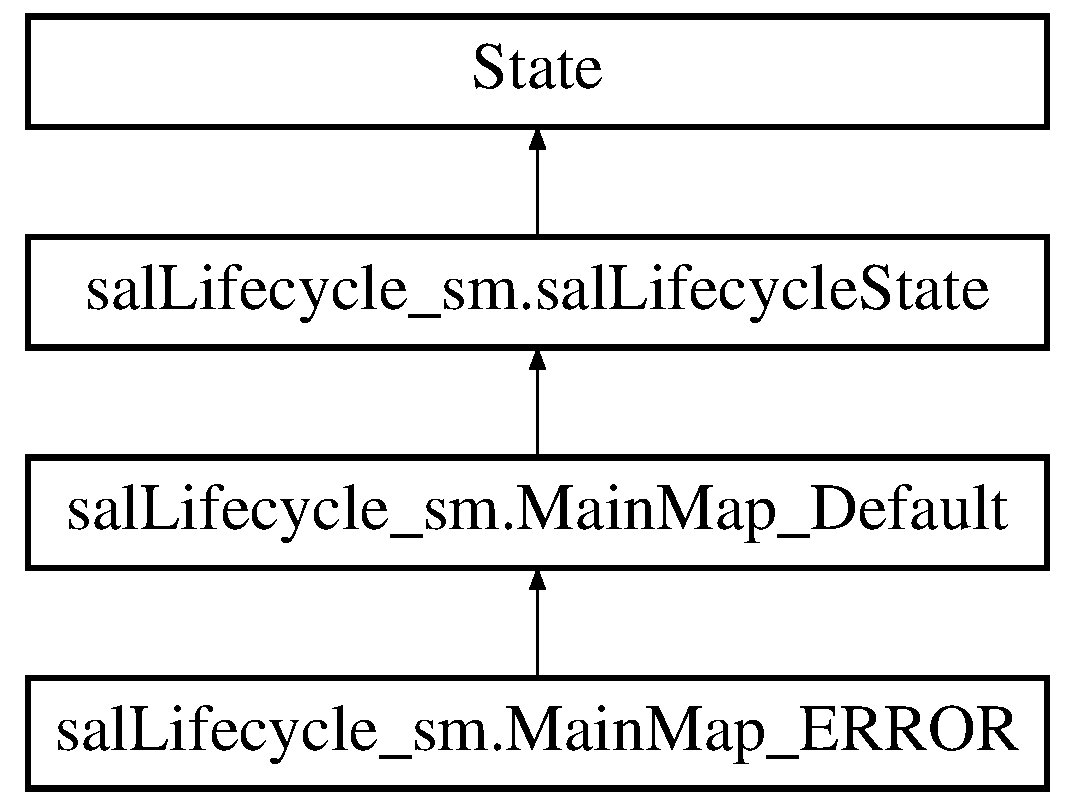
\includegraphics[height=4.000000cm]{classsal_lifecycle__sm_1_1_main_map___e_r_r_o_r}
\end{center}
\end{figure}
\subsection*{Public Member Functions}
\begin{DoxyCompactItemize}
\item 
\hypertarget{classsal_lifecycle__sm_1_1_main_map___e_r_r_o_r_aa63440a6eb00f1324bb1095b03b22df1}{def {\bfseries ocs\-Reset}}\label{classsal_lifecycle__sm_1_1_main_map___e_r_r_o_r_aa63440a6eb00f1324bb1095b03b22df1}

\end{DoxyCompactItemize}


\subsection{Detailed Description}


Definition at line 227 of file sal\-Lifecycle\-\_\-sm.\-py.



The documentation for this class was generated from the following file\-:\begin{DoxyCompactItemize}
\item 
/opt/lsstsal/state\-Machine/python/sal\-Lifecycle\-\_\-sm.\-py\end{DoxyCompactItemize}

\hypertarget{class_main_map___off}{\section{Main\-Map\-\_\-\-Off Class Reference}
\label{class_main_map___off}\index{Main\-Map\-\_\-\-Off@{Main\-Map\-\_\-\-Off}}
}
Inheritance diagram for Main\-Map\-\_\-\-Off\-:\begin{figure}[H]
\begin{center}
\leavevmode
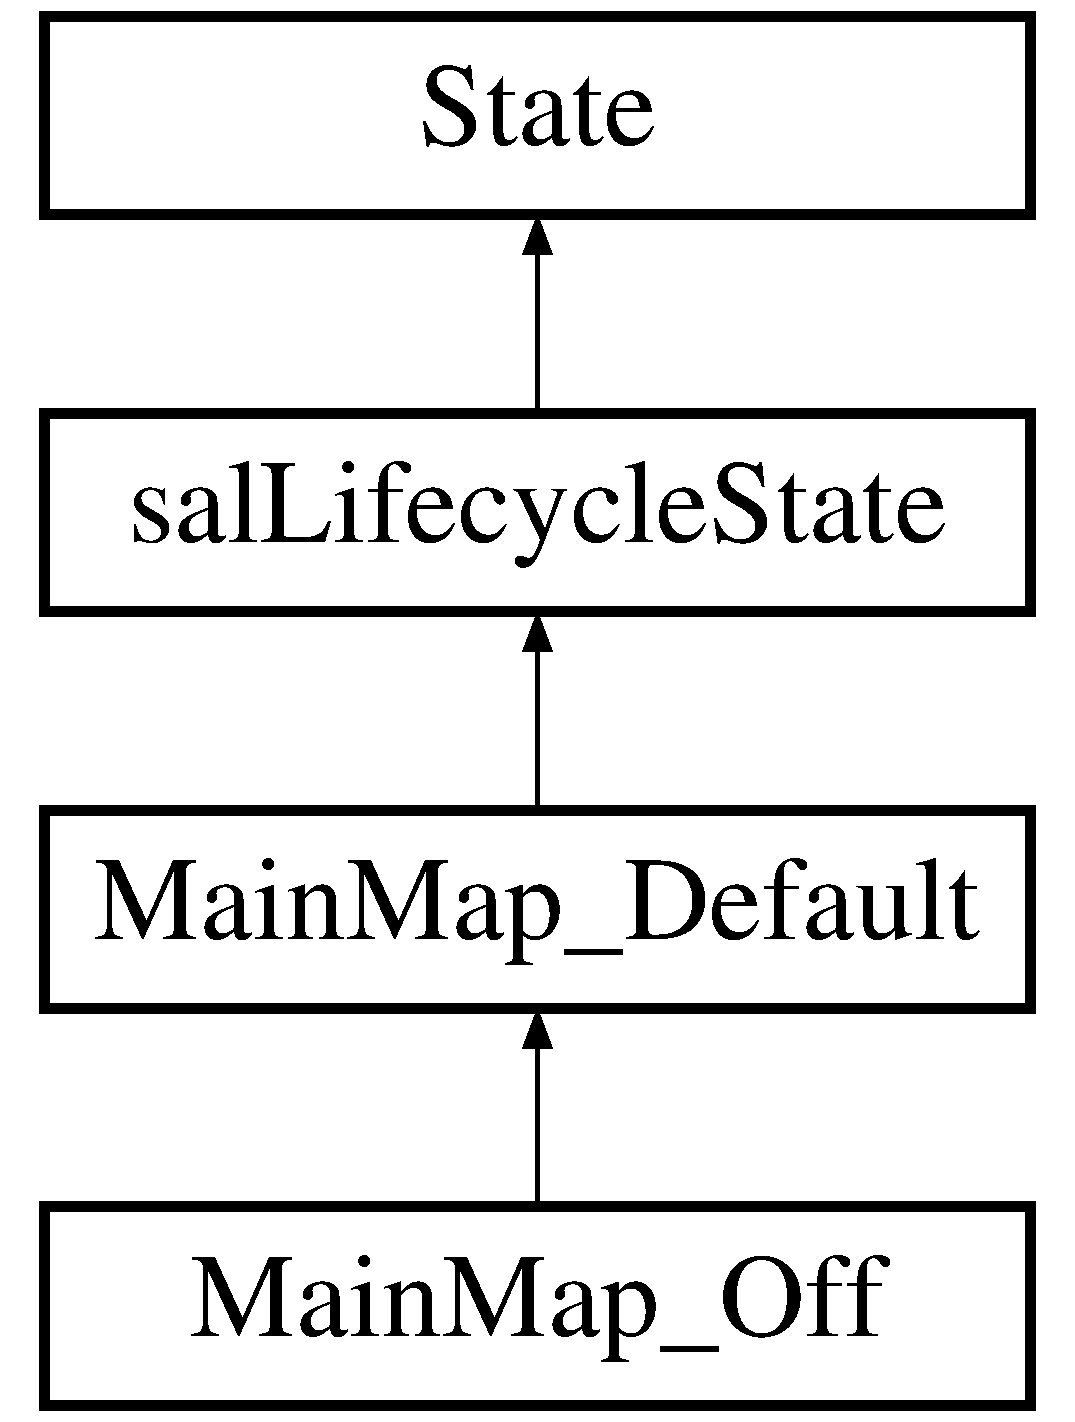
\includegraphics[height=4.000000cm]{class_main_map___off}
\end{center}
\end{figure}
\subsection*{Public Member Functions}
\begin{DoxyCompactItemize}
\item 
\hypertarget{class_main_map___off_aa3e9af24237a529b03889d60940e0978}{{\bfseries Main\-Map\-\_\-\-Off} (const char $\ast$const name, const int state\-Id)}\label{class_main_map___off_aa3e9af24237a529b03889d60940e0978}

\item 
\hypertarget{class_main_map___off_a4a3455c2ffd13127617567c9d617e898}{virtual void {\bfseries ocs\-Boot} (sal\-Lifecycle-\/\hyperlink{classcpp_context}{cpp\-Context} \&context)}\label{class_main_map___off_a4a3455c2ffd13127617567c9d617e898}

\end{DoxyCompactItemize}
\subsection*{Additional Inherited Members}


\subsection{Detailed Description}


Definition at line 84 of file sal\-Lifecycle-\/cpp\-\_\-sm.\-h.



The documentation for this class was generated from the following files\-:\begin{DoxyCompactItemize}
\item 
/opt/lsstsal/state\-Machine/cpp/sal\-Lifecycle-\/cpp\-\_\-sm.\-h\item 
/opt/lsstsal/state\-Machine/cpp/sal\-Lifecycle-\/cpp\-\_\-sm.\-cpp\end{DoxyCompactItemize}

\hypertarget{classsal_lifecycle__sm_1_1_main_map___off}{\section{sal\-Lifecycle\-\_\-sm.\-Main\-Map\-\_\-\-Off Class Reference}
\label{classsal_lifecycle__sm_1_1_main_map___off}\index{sal\-Lifecycle\-\_\-sm.\-Main\-Map\-\_\-\-Off@{sal\-Lifecycle\-\_\-sm.\-Main\-Map\-\_\-\-Off}}
}
Inheritance diagram for sal\-Lifecycle\-\_\-sm.\-Main\-Map\-\_\-\-Off\-:\begin{figure}[H]
\begin{center}
\leavevmode
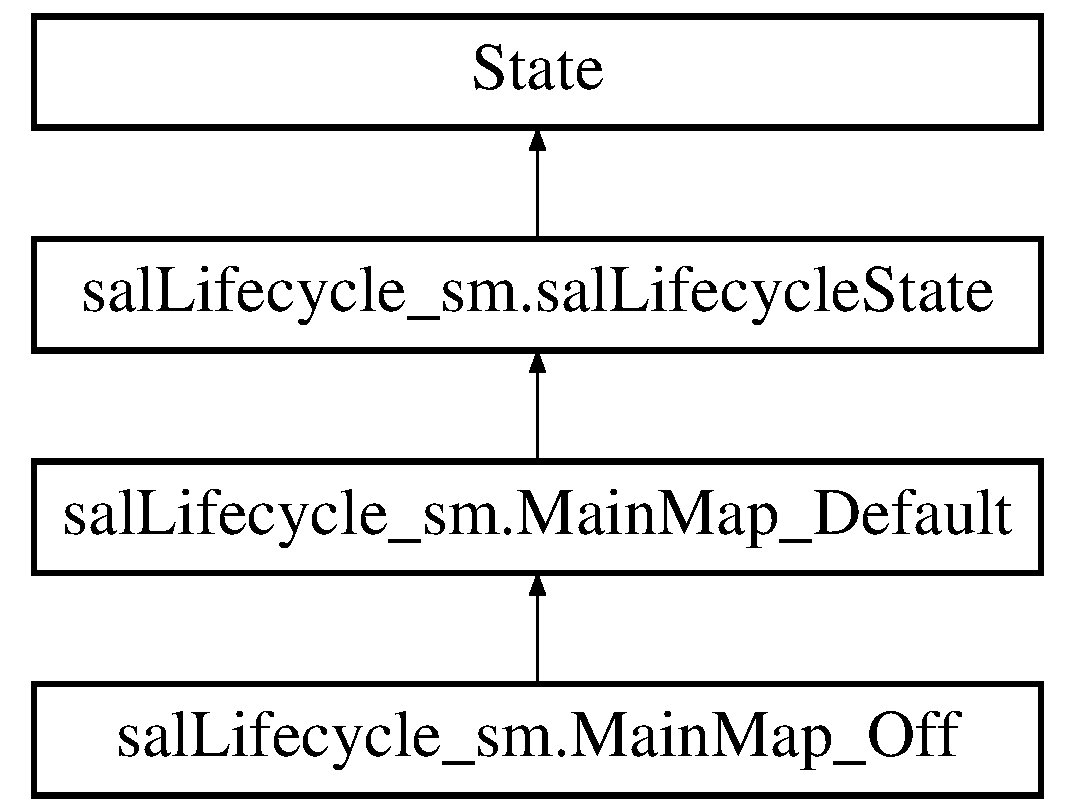
\includegraphics[height=4.000000cm]{classsal_lifecycle__sm_1_1_main_map___off}
\end{center}
\end{figure}
\subsection*{Public Member Functions}
\begin{DoxyCompactItemize}
\item 
\hypertarget{classsal_lifecycle__sm_1_1_main_map___off_aec35ac388d0f057979885f845f15d732}{def {\bfseries ocs\-Boot}}\label{classsal_lifecycle__sm_1_1_main_map___off_aec35ac388d0f057979885f845f15d732}

\end{DoxyCompactItemize}


\subsection{Detailed Description}


Definition at line 67 of file sal\-Lifecycle\-\_\-sm.\-py.



The documentation for this class was generated from the following file\-:\begin{DoxyCompactItemize}
\item 
/opt/lsstsal/state\-Machine/python/sal\-Lifecycle\-\_\-sm.\-py\end{DoxyCompactItemize}

\hypertarget{class_main_map___s_t_a_n_d_b_y}{\section{Main\-Map\-\_\-\-S\-T\-A\-N\-D\-B\-Y Class Reference}
\label{class_main_map___s_t_a_n_d_b_y}\index{Main\-Map\-\_\-\-S\-T\-A\-N\-D\-B\-Y@{Main\-Map\-\_\-\-S\-T\-A\-N\-D\-B\-Y}}
}
Inheritance diagram for Main\-Map\-\_\-\-S\-T\-A\-N\-D\-B\-Y\-:\begin{figure}[H]
\begin{center}
\leavevmode
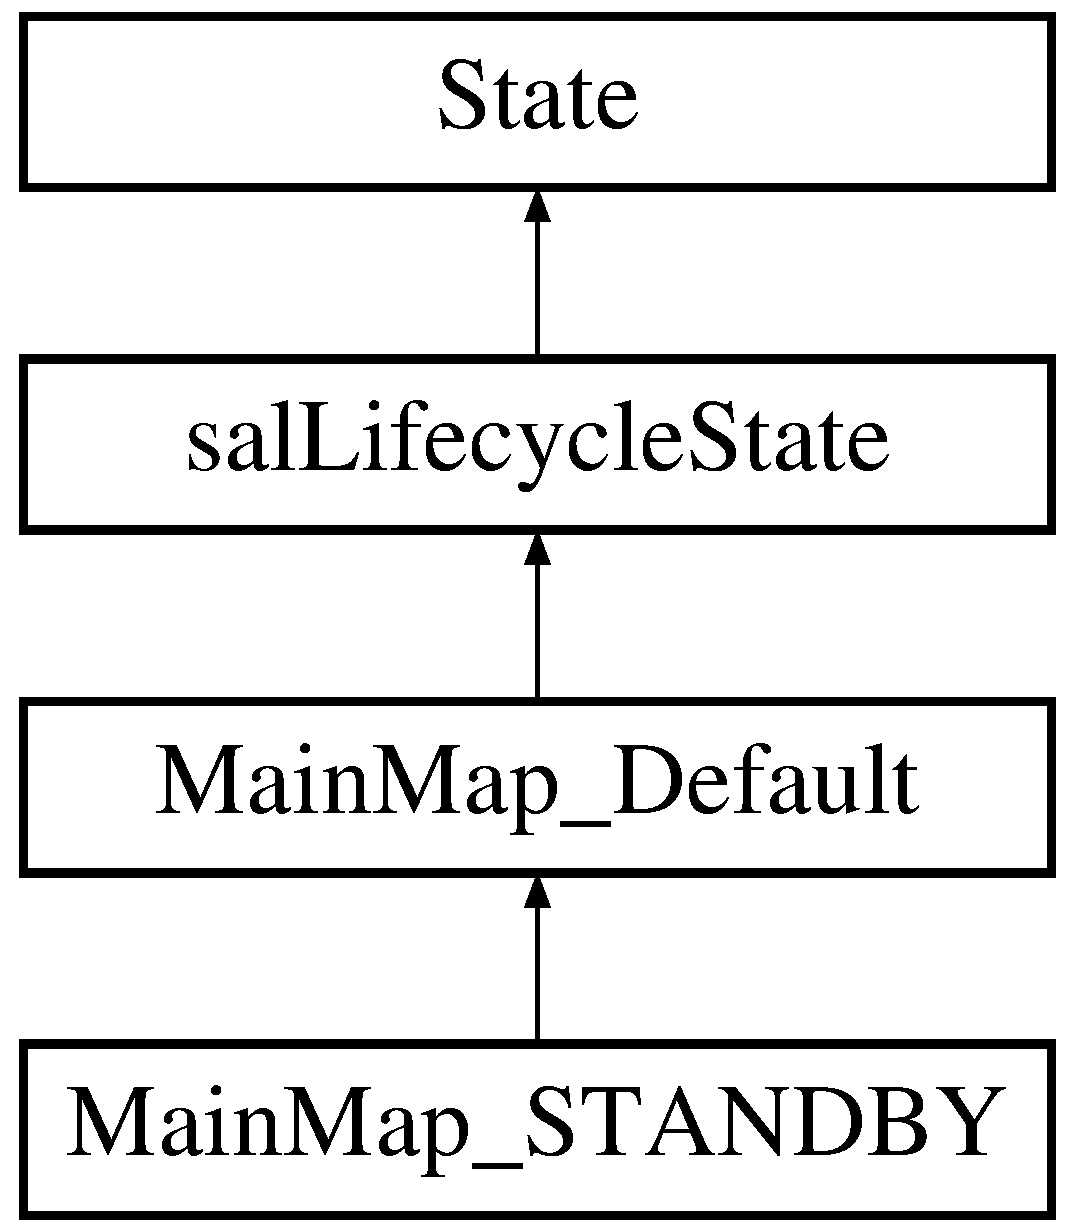
\includegraphics[height=4.000000cm]{class_main_map___s_t_a_n_d_b_y}
\end{center}
\end{figure}
\subsection*{Public Member Functions}
\begin{DoxyCompactItemize}
\item 
\hypertarget{class_main_map___s_t_a_n_d_b_y_abc2f5c4032267303b76ea7cc824f5e1b}{{\bfseries Main\-Map\-\_\-\-S\-T\-A\-N\-D\-B\-Y} (const char $\ast$const name, const int state\-Id)}\label{class_main_map___s_t_a_n_d_b_y_abc2f5c4032267303b76ea7cc824f5e1b}

\item 
\hypertarget{class_main_map___s_t_a_n_d_b_y_ad57727d529180983d334e02e9a0642d7}{virtual void {\bfseries ocs\-Configure} (sal\-Lifecycle-\/\hyperlink{classcpp_context}{cpp\-Context} \&context)}\label{class_main_map___s_t_a_n_d_b_y_ad57727d529180983d334e02e9a0642d7}

\item 
\hypertarget{class_main_map___s_t_a_n_d_b_y_adf5c00d0f404320a293bc9e3d6646231}{virtual void {\bfseries ocs\-Quit} (sal\-Lifecycle-\/\hyperlink{classcpp_context}{cpp\-Context} \&context)}\label{class_main_map___s_t_a_n_d_b_y_adf5c00d0f404320a293bc9e3d6646231}

\end{DoxyCompactItemize}
\subsection*{Additional Inherited Members}


\subsection{Detailed Description}


Definition at line 95 of file sal\-Lifecycle-\/cpp\-\_\-sm.\-h.



The documentation for this class was generated from the following files\-:\begin{DoxyCompactItemize}
\item 
/opt/lsstsal/state\-Machine/cpp/sal\-Lifecycle-\/cpp\-\_\-sm.\-h\item 
/opt/lsstsal/state\-Machine/cpp/sal\-Lifecycle-\/cpp\-\_\-sm.\-cpp\end{DoxyCompactItemize}

\hypertarget{classsal_lifecycle__sm_1_1_main_map___s_t_a_n_d_b_y}{\section{sal\-Lifecycle\-\_\-sm.\-Main\-Map\-\_\-\-S\-T\-A\-N\-D\-B\-Y Class Reference}
\label{classsal_lifecycle__sm_1_1_main_map___s_t_a_n_d_b_y}\index{sal\-Lifecycle\-\_\-sm.\-Main\-Map\-\_\-\-S\-T\-A\-N\-D\-B\-Y@{sal\-Lifecycle\-\_\-sm.\-Main\-Map\-\_\-\-S\-T\-A\-N\-D\-B\-Y}}
}
Inheritance diagram for sal\-Lifecycle\-\_\-sm.\-Main\-Map\-\_\-\-S\-T\-A\-N\-D\-B\-Y\-:\begin{figure}[H]
\begin{center}
\leavevmode
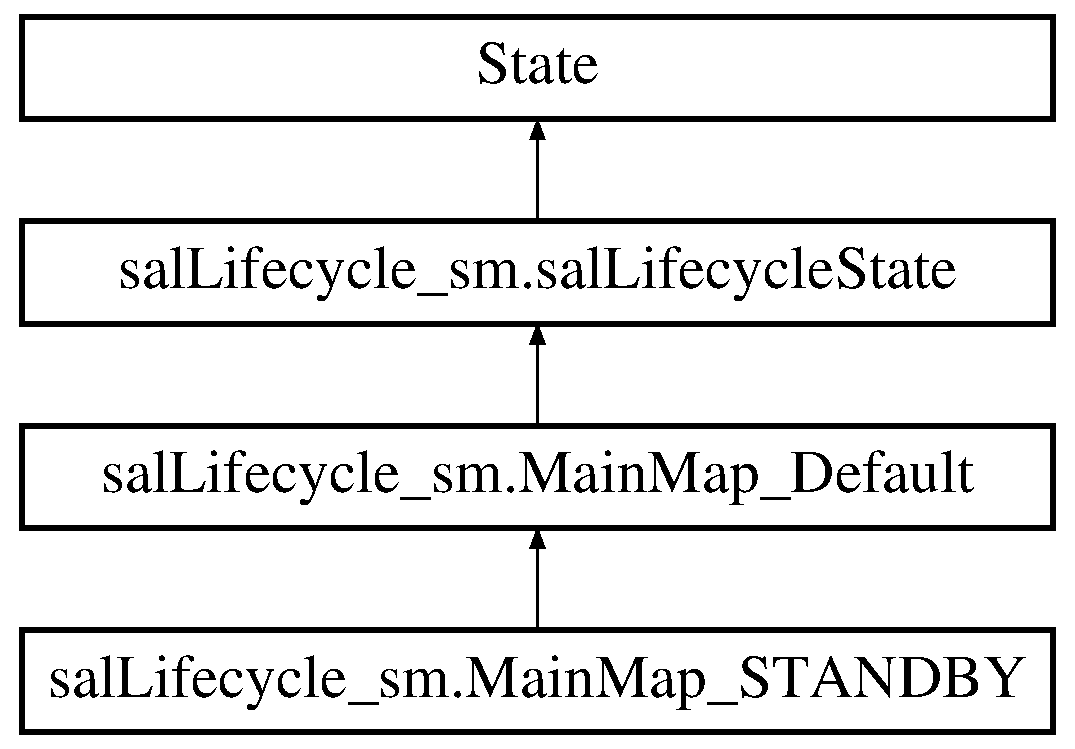
\includegraphics[height=4.000000cm]{classsal_lifecycle__sm_1_1_main_map___s_t_a_n_d_b_y}
\end{center}
\end{figure}
\subsection*{Public Member Functions}
\begin{DoxyCompactItemize}
\item 
\hypertarget{classsal_lifecycle__sm_1_1_main_map___s_t_a_n_d_b_y_ac44fd76aaf23c2d75885086bf0e5f024}{def {\bfseries ocs\-Configure}}\label{classsal_lifecycle__sm_1_1_main_map___s_t_a_n_d_b_y_ac44fd76aaf23c2d75885086bf0e5f024}

\item 
\hypertarget{classsal_lifecycle__sm_1_1_main_map___s_t_a_n_d_b_y_a7005de02474d9e0affb8c94b5d7c08e9}{def {\bfseries ocs\-Quit}}\label{classsal_lifecycle__sm_1_1_main_map___s_t_a_n_d_b_y_a7005de02474d9e0affb8c94b5d7c08e9}

\end{DoxyCompactItemize}


\subsection{Detailed Description}


Definition at line 79 of file sal\-Lifecycle\-\_\-sm.\-py.



The documentation for this class was generated from the following file\-:\begin{DoxyCompactItemize}
\item 
/opt/lsstsal/state\-Machine/python/sal\-Lifecycle\-\_\-sm.\-py\end{DoxyCompactItemize}

\hypertarget{classsal_lifecycle__sm_1_1sal_lifecycle__sm}{\section{sal\-Lifecycle\-\_\-sm.\-sal\-Lifecycle\-\_\-sm Class Reference}
\label{classsal_lifecycle__sm_1_1sal_lifecycle__sm}\index{sal\-Lifecycle\-\_\-sm.\-sal\-Lifecycle\-\_\-sm@{sal\-Lifecycle\-\_\-sm.\-sal\-Lifecycle\-\_\-sm}}
}
Inheritance diagram for sal\-Lifecycle\-\_\-sm.\-sal\-Lifecycle\-\_\-sm\-:\begin{figure}[H]
\begin{center}
\leavevmode
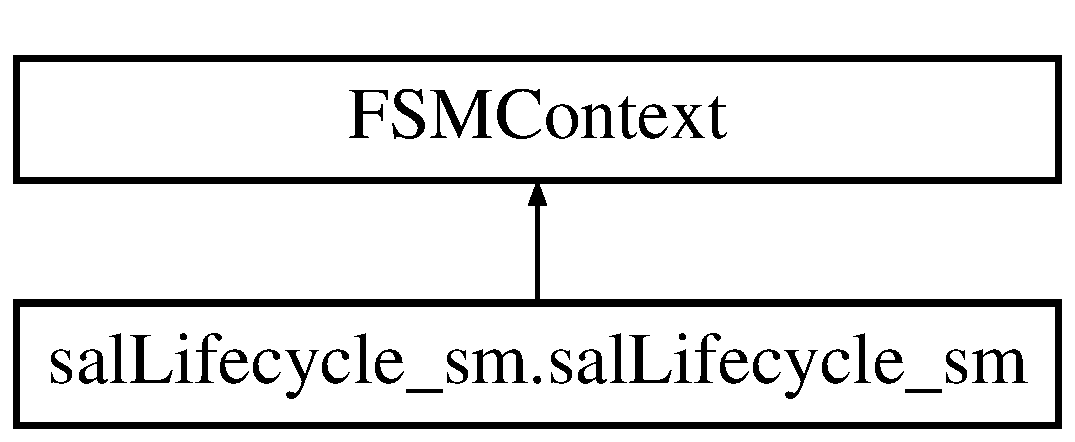
\includegraphics[height=2.000000cm]{classsal_lifecycle__sm_1_1sal_lifecycle__sm}
\end{center}
\end{figure}
\subsection*{Public Member Functions}
\begin{DoxyCompactItemize}
\item 
\hypertarget{classsal_lifecycle__sm_1_1sal_lifecycle__sm_a3f2d1ee1c4f6625ccc008f1d10fac4ab}{def {\bfseries \-\_\-\-\_\-init\-\_\-\-\_\-}}\label{classsal_lifecycle__sm_1_1sal_lifecycle__sm_a3f2d1ee1c4f6625ccc008f1d10fac4ab}

\item 
\hypertarget{classsal_lifecycle__sm_1_1sal_lifecycle__sm_aef34790057f8ab81af6217354793e0b1}{def {\bfseries \-\_\-\-\_\-getattr\-\_\-\-\_\-}}\label{classsal_lifecycle__sm_1_1sal_lifecycle__sm_aef34790057f8ab81af6217354793e0b1}

\item 
\hypertarget{classsal_lifecycle__sm_1_1sal_lifecycle__sm_a1e0a078e9ba8723f33ce6e89f478bff8}{def {\bfseries enter\-Start\-State}}\label{classsal_lifecycle__sm_1_1sal_lifecycle__sm_a1e0a078e9ba8723f33ce6e89f478bff8}

\item 
\hypertarget{classsal_lifecycle__sm_1_1sal_lifecycle__sm_a0e902cb5dd1524880a0e2753ecde7fec}{def {\bfseries get\-Owner}}\label{classsal_lifecycle__sm_1_1sal_lifecycle__sm_a0e902cb5dd1524880a0e2753ecde7fec}

\end{DoxyCompactItemize}


\subsection{Detailed Description}


Definition at line 249 of file sal\-Lifecycle\-\_\-sm.\-py.



The documentation for this class was generated from the following file\-:\begin{DoxyCompactItemize}
\item 
/opt/lsstsal/state\-Machine/python/sal\-Lifecycle\-\_\-sm.\-py\end{DoxyCompactItemize}

\hypertarget{classsal_lifecycle_context}{\section{sal\-Lifecycle\-Context Class Reference}
\label{classsal_lifecycle_context}\index{sal\-Lifecycle\-Context@{sal\-Lifecycle\-Context}}
}
Inheritance diagram for sal\-Lifecycle\-Context\-:\begin{figure}[H]
\begin{center}
\leavevmode
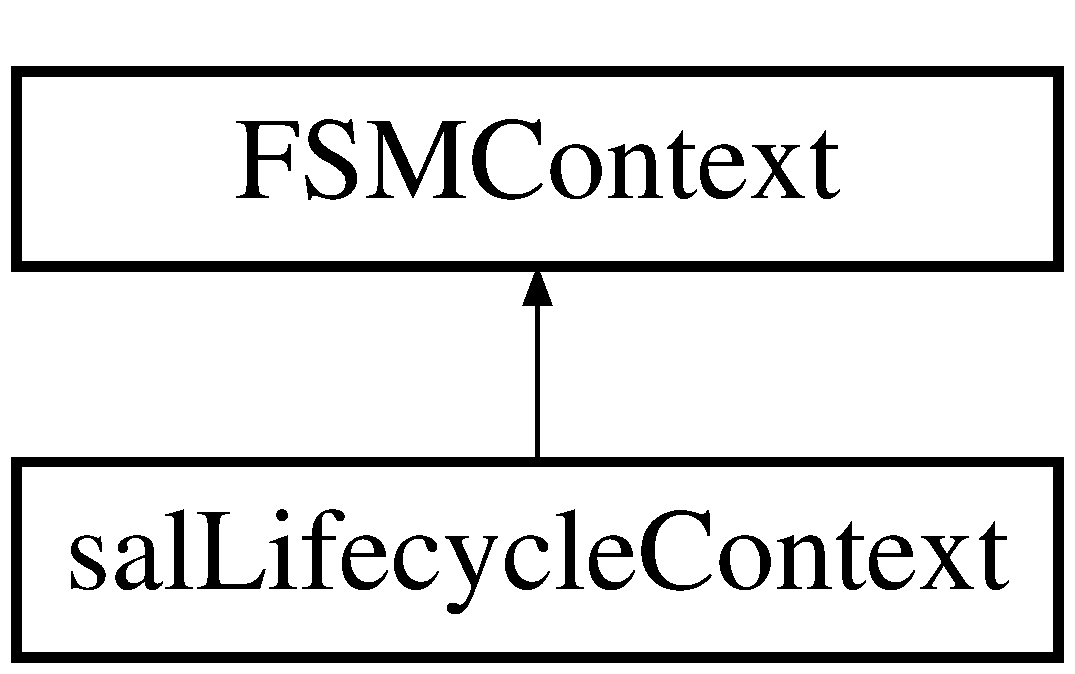
\includegraphics[height=2.000000cm]{classsal_lifecycle_context}
\end{center}
\end{figure}
\subsection*{Classes}
\begin{DoxyCompactItemize}
\item 
class {\bfseries Main\-Map}
\item 
class {\bfseries Main\-Map\-\_\-\-Default}
\item 
class {\bfseries sal\-Lifecycle\-State}
\end{DoxyCompactItemize}
\subsection*{Public Member Functions}
\begin{DoxyCompactItemize}
\item 
\hypertarget{classsal_lifecycle_context_a0bf4c186610c050a53427ae2ef5d3ffb}{{\bfseries sal\-Lifecycle\-Context} (sal\-Lifecycle owner)}\label{classsal_lifecycle_context_a0bf4c186610c050a53427ae2ef5d3ffb}

\item 
\hypertarget{classsal_lifecycle_context_a7f84069ab0d79e2cd81f7990a329b1e6}{{\bfseries sal\-Lifecycle\-Context} (sal\-Lifecycle owner, \hyperlink{classsal_lifecycle_state}{sal\-Lifecycle\-State} init\-State)}\label{classsal_lifecycle_context_a7f84069ab0d79e2cd81f7990a329b1e6}

\item 
\hypertarget{classsal_lifecycle_context_a8e57d270e6741d105a52a4f2508ea884}{void {\bfseries enter\-Start\-State} ()}\label{classsal_lifecycle_context_a8e57d270e6741d105a52a4f2508ea884}

\item 
\hypertarget{classsal_lifecycle_context_ac136c14aef8923874e83596679ca5221}{void {\bfseries configure\-Error} ()}\label{classsal_lifecycle_context_ac136c14aef8923874e83596679ca5221}

\item 
\hypertarget{classsal_lifecycle_context_a610552ef7ed4a54fd4707c75ae7cb338}{void {\bfseries disable\-Error} ()}\label{classsal_lifecycle_context_a610552ef7ed4a54fd4707c75ae7cb338}

\item 
\hypertarget{classsal_lifecycle_context_acea6cc163e624c7abe7e5b6b894416bd}{void {\bfseries enable\-Error} ()}\label{classsal_lifecycle_context_acea6cc163e624c7abe7e5b6b894416bd}

\item 
\hypertarget{classsal_lifecycle_context_a49d10bc8f396d4844fc13b7416f43a6e}{void {\bfseries ocs\-Abandon} ()}\label{classsal_lifecycle_context_a49d10bc8f396d4844fc13b7416f43a6e}

\item 
\hypertarget{classsal_lifecycle_context_a476935dbecb6ee4f238341464785dcea}{void {\bfseries ocs\-Abort} ()}\label{classsal_lifecycle_context_a476935dbecb6ee4f238341464785dcea}

\item 
\hypertarget{classsal_lifecycle_context_ab8f06491f6e375e6f9a0aa0f15853a5a}{void {\bfseries ocs\-Boot} ()}\label{classsal_lifecycle_context_ab8f06491f6e375e6f9a0aa0f15853a5a}

\item 
\hypertarget{classsal_lifecycle_context_a3f8c0a280d38bbb4a1a5d8d22490844e}{void {\bfseries ocs\-Configure} ()}\label{classsal_lifecycle_context_a3f8c0a280d38bbb4a1a5d8d22490844e}

\item 
\hypertarget{classsal_lifecycle_context_aa091643e8f189b1cbf7584a9944e6e64}{void {\bfseries ocs\-Disable} ()}\label{classsal_lifecycle_context_aa091643e8f189b1cbf7584a9944e6e64}

\item 
\hypertarget{classsal_lifecycle_context_a3cbbd9a3b6613764d6f341a8c72b5aa8}{void {\bfseries ocs\-Enable} ()}\label{classsal_lifecycle_context_a3cbbd9a3b6613764d6f341a8c72b5aa8}

\item 
\hypertarget{classsal_lifecycle_context_ae9fbaf60dee7565329aae5db085b069b}{void {\bfseries ocs\-Quit} ()}\label{classsal_lifecycle_context_ae9fbaf60dee7565329aae5db085b069b}

\item 
\hypertarget{classsal_lifecycle_context_a368e8a292ad623f67187219a3dc2eca1}{void {\bfseries ocs\-Reset} ()}\label{classsal_lifecycle_context_a368e8a292ad623f67187219a3dc2eca1}

\item 
\hypertarget{classsal_lifecycle_context_a10ca8dcf34e175612db7f3cce421343d}{void {\bfseries ocs\-Set\-Value} ()}\label{classsal_lifecycle_context_a10ca8dcf34e175612db7f3cce421343d}

\item 
\hypertarget{classsal_lifecycle_context_a84c110a3e22e2f9b649fbbf479007b0b}{void {\bfseries ocs\-Stop} ()}\label{classsal_lifecycle_context_a84c110a3e22e2f9b649fbbf479007b0b}

\item 
\hypertarget{classsal_lifecycle_context_a4f5c224ef8b4b16e4824c47ce2bb89de}{void {\bfseries ocs\-Un\-Configure} ()}\label{classsal_lifecycle_context_a4f5c224ef8b4b16e4824c47ce2bb89de}

\item 
\hypertarget{classsal_lifecycle_context_aaff1ef965fa37e8afbe77ddabef6350c}{\hyperlink{classsal_lifecycle_state}{sal\-Lifecycle\-State} {\bfseries get\-State} ()  throws statemap.\-State\-Undefined\-Exception     }\label{classsal_lifecycle_context_aaff1ef965fa37e8afbe77ddabef6350c}

\item 
\hypertarget{classsal_lifecycle_context_a465b41ff56477227b1beecdebaa3d655}{void {\bfseries set\-Owner} (sal\-Lifecycle owner)}\label{classsal_lifecycle_context_a465b41ff56477227b1beecdebaa3d655}

\end{DoxyCompactItemize}
\subsection*{Protected Member Functions}
\begin{DoxyCompactItemize}
\item 
\hypertarget{classsal_lifecycle_context_ad2f47a1d339cbe171ddb73213290b1e5}{sal\-Lifecycle {\bfseries get\-Owner} ()}\label{classsal_lifecycle_context_ad2f47a1d339cbe171ddb73213290b1e5}

\end{DoxyCompactItemize}


\subsection{Detailed Description}


Definition at line 9 of file sal\-Lifecycle\-Context.\-java.



The documentation for this class was generated from the following file\-:\begin{DoxyCompactItemize}
\item 
/opt/lsstsal/state\-Machine/java/sal\-Lifecycle\-Context.\-java\end{DoxyCompactItemize}

\hypertarget{classsal_lifecycle__sm_1_1sal_lifecycle_state}{\section{sal\-Lifecycle\-\_\-sm.\-sal\-Lifecycle\-State Class Reference}
\label{classsal_lifecycle__sm_1_1sal_lifecycle_state}\index{sal\-Lifecycle\-\_\-sm.\-sal\-Lifecycle\-State@{sal\-Lifecycle\-\_\-sm.\-sal\-Lifecycle\-State}}
}
Inheritance diagram for sal\-Lifecycle\-\_\-sm.\-sal\-Lifecycle\-State\-:\begin{figure}[H]
\begin{center}
\leavevmode
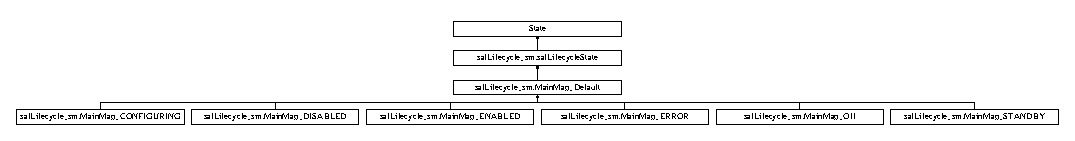
\includegraphics[height=1.441441cm]{classsal_lifecycle__sm_1_1sal_lifecycle_state}
\end{center}
\end{figure}
\subsection*{Public Member Functions}
\begin{DoxyCompactItemize}
\item 
\hypertarget{classsal_lifecycle__sm_1_1sal_lifecycle_state_ad26f7101495c09dcd24bdf6b2c8fab07}{def {\bfseries Entry}}\label{classsal_lifecycle__sm_1_1sal_lifecycle_state_ad26f7101495c09dcd24bdf6b2c8fab07}

\item 
\hypertarget{classsal_lifecycle__sm_1_1sal_lifecycle_state_ae9a2382adbb05e0779e57e1dc55f3714}{def {\bfseries Exit}}\label{classsal_lifecycle__sm_1_1sal_lifecycle_state_ae9a2382adbb05e0779e57e1dc55f3714}

\item 
\hypertarget{classsal_lifecycle__sm_1_1sal_lifecycle_state_a9c560318f86a782546da136c2d50e776}{def {\bfseries configure\-Error}}\label{classsal_lifecycle__sm_1_1sal_lifecycle_state_a9c560318f86a782546da136c2d50e776}

\item 
\hypertarget{classsal_lifecycle__sm_1_1sal_lifecycle_state_a84ce90618b90fd89f928f55f4e14c61f}{def {\bfseries disable\-Error}}\label{classsal_lifecycle__sm_1_1sal_lifecycle_state_a84ce90618b90fd89f928f55f4e14c61f}

\item 
\hypertarget{classsal_lifecycle__sm_1_1sal_lifecycle_state_a668826955e8ab9aba9f60620f20e2a7b}{def {\bfseries enable\-Error}}\label{classsal_lifecycle__sm_1_1sal_lifecycle_state_a668826955e8ab9aba9f60620f20e2a7b}

\item 
\hypertarget{classsal_lifecycle__sm_1_1sal_lifecycle_state_a2fbbcd8746f3069880f8bc3d3bfc8793}{def {\bfseries ocs\-Abandon}}\label{classsal_lifecycle__sm_1_1sal_lifecycle_state_a2fbbcd8746f3069880f8bc3d3bfc8793}

\item 
\hypertarget{classsal_lifecycle__sm_1_1sal_lifecycle_state_a0a00222c2d2a013a0d9dc79dcf5b1f3d}{def {\bfseries ocs\-Abort}}\label{classsal_lifecycle__sm_1_1sal_lifecycle_state_a0a00222c2d2a013a0d9dc79dcf5b1f3d}

\item 
\hypertarget{classsal_lifecycle__sm_1_1sal_lifecycle_state_aec76b1d3843764ca1fd1fff2d2ed4191}{def {\bfseries ocs\-Boot}}\label{classsal_lifecycle__sm_1_1sal_lifecycle_state_aec76b1d3843764ca1fd1fff2d2ed4191}

\item 
\hypertarget{classsal_lifecycle__sm_1_1sal_lifecycle_state_a5da676c49f4f1fa25af8adb85713fa1a}{def {\bfseries ocs\-Configure}}\label{classsal_lifecycle__sm_1_1sal_lifecycle_state_a5da676c49f4f1fa25af8adb85713fa1a}

\item 
\hypertarget{classsal_lifecycle__sm_1_1sal_lifecycle_state_af302c5fcd4ff69ee746535b9076dabcf}{def {\bfseries ocs\-Disable}}\label{classsal_lifecycle__sm_1_1sal_lifecycle_state_af302c5fcd4ff69ee746535b9076dabcf}

\item 
\hypertarget{classsal_lifecycle__sm_1_1sal_lifecycle_state_a3fd270a4f1e5617083362eed4d816d0a}{def {\bfseries ocs\-Enable}}\label{classsal_lifecycle__sm_1_1sal_lifecycle_state_a3fd270a4f1e5617083362eed4d816d0a}

\item 
\hypertarget{classsal_lifecycle__sm_1_1sal_lifecycle_state_a7e4677857f4cdf65db7f6034c060503c}{def {\bfseries ocs\-Quit}}\label{classsal_lifecycle__sm_1_1sal_lifecycle_state_a7e4677857f4cdf65db7f6034c060503c}

\item 
\hypertarget{classsal_lifecycle__sm_1_1sal_lifecycle_state_ac048a2fa00c0b849e4f2574d198136ac}{def {\bfseries ocs\-Reset}}\label{classsal_lifecycle__sm_1_1sal_lifecycle_state_ac048a2fa00c0b849e4f2574d198136ac}

\item 
\hypertarget{classsal_lifecycle__sm_1_1sal_lifecycle_state_a02bfbff33f38c7538eb6b9841490391e}{def {\bfseries ocs\-Set\-Value}}\label{classsal_lifecycle__sm_1_1sal_lifecycle_state_a02bfbff33f38c7538eb6b9841490391e}

\item 
\hypertarget{classsal_lifecycle__sm_1_1sal_lifecycle_state_a88fee5c44a603d1de73452386daa6841}{def {\bfseries ocs\-Stop}}\label{classsal_lifecycle__sm_1_1sal_lifecycle_state_a88fee5c44a603d1de73452386daa6841}

\item 
\hypertarget{classsal_lifecycle__sm_1_1sal_lifecycle_state_a31502cc7f0c32a727137f785df514619}{def {\bfseries ocs\-Un\-Configure}}\label{classsal_lifecycle__sm_1_1sal_lifecycle_state_a31502cc7f0c32a727137f785df514619}

\item 
\hypertarget{classsal_lifecycle__sm_1_1sal_lifecycle_state_a61de8d78b48c29b2bbddafa78ff1e7e6}{def {\bfseries Default}}\label{classsal_lifecycle__sm_1_1sal_lifecycle_state_a61de8d78b48c29b2bbddafa78ff1e7e6}

\end{DoxyCompactItemize}


\subsection{Detailed Description}


Definition at line 9 of file sal\-Lifecycle\-\_\-sm.\-py.



The documentation for this class was generated from the following file\-:\begin{DoxyCompactItemize}
\item 
/opt/lsstsal/state\-Machine/python/sal\-Lifecycle\-\_\-sm.\-py\end{DoxyCompactItemize}

\hypertarget{classsal_lifecycle_state}{\section{sal\-Lifecycle\-State Class Reference}
\label{classsal_lifecycle_state}\index{sal\-Lifecycle\-State@{sal\-Lifecycle\-State}}
}
Inheritance diagram for sal\-Lifecycle\-State\-:\begin{figure}[H]
\begin{center}
\leavevmode
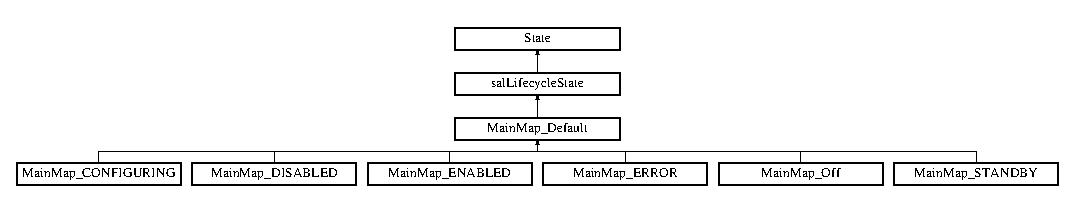
\includegraphics[height=2.262626cm]{classsal_lifecycle_state}
\end{center}
\end{figure}
\subsection*{Public Member Functions}
\begin{DoxyCompactItemize}
\item 
\hypertarget{classsal_lifecycle_state_a76491dca6083f5aeb34eca62e5d7f451}{{\bfseries sal\-Lifecycle\-State} (const char $\ast$const name, const int state\-Id)}\label{classsal_lifecycle_state_a76491dca6083f5aeb34eca62e5d7f451}

\item 
\hypertarget{classsal_lifecycle_state_a90adbd9a0b400c367c168fcb53e57917}{virtual void {\bfseries Entry} (sal\-Lifecycle-\/\hyperlink{classcpp_context}{cpp\-Context} \&)}\label{classsal_lifecycle_state_a90adbd9a0b400c367c168fcb53e57917}

\item 
\hypertarget{classsal_lifecycle_state_a7389a9959d0a925fc214e8fb9033ba12}{virtual void {\bfseries Exit} (sal\-Lifecycle-\/\hyperlink{classcpp_context}{cpp\-Context} \&)}\label{classsal_lifecycle_state_a7389a9959d0a925fc214e8fb9033ba12}

\item 
\hypertarget{classsal_lifecycle_state_a7771b7a868ec60a9818ea49afde0f68a}{virtual void {\bfseries configure\-Error} (sal\-Lifecycle-\/\hyperlink{classcpp_context}{cpp\-Context} \&context)}\label{classsal_lifecycle_state_a7771b7a868ec60a9818ea49afde0f68a}

\item 
\hypertarget{classsal_lifecycle_state_a6b669876e3f4b8d0cb6a1f4d749f613f}{virtual void {\bfseries disable\-Error} (sal\-Lifecycle-\/\hyperlink{classcpp_context}{cpp\-Context} \&context)}\label{classsal_lifecycle_state_a6b669876e3f4b8d0cb6a1f4d749f613f}

\item 
\hypertarget{classsal_lifecycle_state_a664bc49c7dc4e083f60873a99f1ad051}{virtual void {\bfseries enable\-Error} (sal\-Lifecycle-\/\hyperlink{classcpp_context}{cpp\-Context} \&context)}\label{classsal_lifecycle_state_a664bc49c7dc4e083f60873a99f1ad051}

\item 
\hypertarget{classsal_lifecycle_state_a8ae5cd42b3c9f6688ae2bab95d91968c}{virtual void {\bfseries ocs\-Abandon} (sal\-Lifecycle-\/\hyperlink{classcpp_context}{cpp\-Context} \&context)}\label{classsal_lifecycle_state_a8ae5cd42b3c9f6688ae2bab95d91968c}

\item 
\hypertarget{classsal_lifecycle_state_ab7b607557680cfaf74263a90f5be39d5}{virtual void {\bfseries ocs\-Abort} (sal\-Lifecycle-\/\hyperlink{classcpp_context}{cpp\-Context} \&context)}\label{classsal_lifecycle_state_ab7b607557680cfaf74263a90f5be39d5}

\item 
\hypertarget{classsal_lifecycle_state_a9ab926e0208ddb776b012647a4f63438}{virtual void {\bfseries ocs\-Boot} (sal\-Lifecycle-\/\hyperlink{classcpp_context}{cpp\-Context} \&context)}\label{classsal_lifecycle_state_a9ab926e0208ddb776b012647a4f63438}

\item 
\hypertarget{classsal_lifecycle_state_a5567e67a9924d644e1a5e7ecd2e510ba}{virtual void {\bfseries ocs\-Configure} (sal\-Lifecycle-\/\hyperlink{classcpp_context}{cpp\-Context} \&context)}\label{classsal_lifecycle_state_a5567e67a9924d644e1a5e7ecd2e510ba}

\item 
\hypertarget{classsal_lifecycle_state_a057a54af03f171a32c609c27873c9621}{virtual void {\bfseries ocs\-Disable} (sal\-Lifecycle-\/\hyperlink{classcpp_context}{cpp\-Context} \&context)}\label{classsal_lifecycle_state_a057a54af03f171a32c609c27873c9621}

\item 
\hypertarget{classsal_lifecycle_state_a2e3a3ee7c4ae90d667a760c695b1ee79}{virtual void {\bfseries ocs\-Enable} (sal\-Lifecycle-\/\hyperlink{classcpp_context}{cpp\-Context} \&context)}\label{classsal_lifecycle_state_a2e3a3ee7c4ae90d667a760c695b1ee79}

\item 
\hypertarget{classsal_lifecycle_state_a23a3d21ddc47a3613392c479f25dde9e}{virtual void {\bfseries ocs\-Quit} (sal\-Lifecycle-\/\hyperlink{classcpp_context}{cpp\-Context} \&context)}\label{classsal_lifecycle_state_a23a3d21ddc47a3613392c479f25dde9e}

\item 
\hypertarget{classsal_lifecycle_state_aefad5dda230a21380d5a6557109b8c53}{virtual void {\bfseries ocs\-Reset} (sal\-Lifecycle-\/\hyperlink{classcpp_context}{cpp\-Context} \&context)}\label{classsal_lifecycle_state_aefad5dda230a21380d5a6557109b8c53}

\item 
\hypertarget{classsal_lifecycle_state_a9b6e16ab531778811762f52caa1954a8}{virtual void {\bfseries ocs\-Set\-Value} (sal\-Lifecycle-\/\hyperlink{classcpp_context}{cpp\-Context} \&context)}\label{classsal_lifecycle_state_a9b6e16ab531778811762f52caa1954a8}

\item 
\hypertarget{classsal_lifecycle_state_ac696e1695290bf25509a2a00109f79ff}{virtual void {\bfseries ocs\-Stop} (sal\-Lifecycle-\/\hyperlink{classcpp_context}{cpp\-Context} \&context)}\label{classsal_lifecycle_state_ac696e1695290bf25509a2a00109f79ff}

\item 
\hypertarget{classsal_lifecycle_state_ae1fad2410fc68567391b866bcf6844ad}{virtual void {\bfseries ocs\-Un\-Configure} (sal\-Lifecycle-\/\hyperlink{classcpp_context}{cpp\-Context} \&context)}\label{classsal_lifecycle_state_ae1fad2410fc68567391b866bcf6844ad}

\end{DoxyCompactItemize}
\subsection*{Protected Member Functions}
\begin{DoxyCompactItemize}
\item 
\hypertarget{classsal_lifecycle_state_a7a2cd66b55e59dd8d1cab519ea90544d}{virtual void {\bfseries Default} (sal\-Lifecycle-\/\hyperlink{classcpp_context}{cpp\-Context} \&context)}\label{classsal_lifecycle_state_a7a2cd66b55e59dd8d1cab519ea90544d}

\end{DoxyCompactItemize}


\subsection{Detailed Description}


Definition at line 29 of file sal\-Lifecycle-\/cpp\-\_\-sm.\-h.



The documentation for this class was generated from the following files\-:\begin{DoxyCompactItemize}
\item 
/opt/lsstsal/state\-Machine/cpp/sal\-Lifecycle-\/cpp\-\_\-sm.\-h\item 
/opt/lsstsal/state\-Machine/cpp/sal\-Lifecycle-\/cpp\-\_\-sm.\-cpp\end{DoxyCompactItemize}

%--- End generated contents ---

% Index
\newpage
\phantomsection
\addcontentsline{toc}{chapter}{Index}
\printindex

\end{document}
